\applynumberofpages\chapter{Instruction Selection}
\chapterauthor{D. Ebner and A. Krall and B. Scholz}
\graphicspath{{fig/}{code_selection/fig/}{part4/code_selection/fig/}}
% some frequently used macros
%%%%%%%%%%%%%%%%%%%%%%%%%%%%%%%%%%%%%%%%%%%%%%%%%%%%%%%%%%%%%%%%%%%%%
\newcommand{\eg}{e.g.\xspace}
\newcommand{\ie}{i.e.\xspace}
\newcommand{\cf}{c.f.\xspace}
\newcommand{\ea}{et~al.\xspace}

\newcommand{\preds}{\emph{preds}}
\newcommand{\succs}{\emph{succs}}
\newcommand{\costs}{\emph{costs}}
\newcommand{\tbd}[1]{\begin{itemize}\item#1\end{itemize}}
\newcommand\vardomain{\mathbb D}
\newcommand\matrixfont{\mathcal}
\newcommand\kw[1]{\textbf{#1}}

\newcommand\cfgnodes{\mathcal N}
\newcommand\cfgedges{\mathcal E}
\newcommand\cfgstart{\textbf{s}}
\newcommand\cfgend{\textbf{e}}
\newcommand\cfg{\textit{CFG}}
\newcommand\varset{\mathcal{V}}
\newcommand{\vdef}[1]{\cfgdef({#1})}
\newcommand{\defs}[1]{\mathcal{D}_{#1}}
\newcommand{\live}[1]{\mathcal{L}_{#1}}
\newcommand{\uses}[1]{\mathcal{U}_{#1}}
\newcommand{\pred}[2]{\cfgpred^{#1}_{#2}}
\newcommand\state{\textbf{state}}
\newcommand\bool{\mathbb B}
\newcommand\btrue{\textit{true}}
\newcommand\bfalse{\textit{false}}
\newcommand\transform{\mathbb T}
\newcommand\alive{\textbf{alive}}
\newcommand\Path{\textit{Path}}
\newcommand\Ops{\textit{Ops}}
\newcommand\bigo{\mathcal O}

\renewcommand{\vec}[1]{\overrightarrow{#1}}
\newcommand{\dotcup}{\ensuremath{\mathaccent\cdot\cup}}

% locally used colors (pantone)
%%%%%%%%%%%%%%%%%%%%%%%%%%%%%%%%%%%%%%%%%%%%%%%%%%%%%%%%%%%%%%%%%%%%%
\definecolor{LightBlue}{rgb}{ 0.67578125, 0.84375, 0.8984375 }
\definecolor{LightCoral}{rgb}{ 0.9375, 0.5, 0.5 }
\definecolor{LightCyan}{rgb}{ 0.875, 0.99609375, 0.99609375 }
\definecolor{LightGoldenRodYellow}{rgb}{ 0.9765625, 0.9765625, 0.8203125 }
\definecolor{LightGrey}{rgb}{ 0.82421875, 0.82421875, 0.82421875 }
\definecolor{LightGreen}{rgb}{ 0.5625, 0.9296875, 0.5625 }
\definecolor{LightPink}{rgb}{ 0.99609375, 0.7109375, 0.75390625 }
\definecolor{LightSalmon}{rgb}{ 0.99609375, 0.625, 0.4765625 }
\definecolor{LightSeaGreen}{rgb}{ 0.125, 0.6953125, 0.6640625 }
\definecolor{LightSkyBlue}{rgb}{ 0.52734375, 0.8046875, 0.9765625 }
\definecolor{LightSlateBlue}{rgb}{ 0.515625, 0.4375, 0.99609375 }
\definecolor{LightSlateGray}{rgb}{ 0.46484375, 0.53125, 0.59765625 }
\definecolor{LightSteelBlue}{rgb}{ 0.6875, 0.765625, 0.8671875 }
\definecolor{LightYellow}{rgb}{ 0.99609375, 0.99609375, 0.875 }
\definecolor{Orange}{rgb}{ 0.99609375, 0.64453125, 0.0 }
\definecolor{OrangeRed}{rgb}{ 0.99609375, 0.26953125, 0.0 }
\definecolor{Orchid}{rgb}{ 0.8515625, 0.4375, 0.8359375 }

% tikz styles
%%%%%%%%%%%%%%%%%%%%%%%%%%%%%%%%%%%%%%%%%%%%%%%%%%%%%%%%%%%%%%%%%%%%%
% \tikzstyle{arrow} = [draw,>=triangle 45]
% \tikzstyle{fnode} = [shape=ellipse, draw, minimum width=1.5cm,
%                      minimum height=0.8cm, node distance=1.5cm,
%                      text centered, fill=LightBlue]
\section{Introduction}

Instruction selection is a transformation step in a compiler that
translates a machine-independent intermediate code representation into
a low-level intermediate representation or to machine code for a
specific target architecture. Instead of hand-crafting an instruction
selector for each target architecture, generator tools have been
designed and implemented that generate the instruction selector based
on a specification of the machine description of the target. The study
and implementation of generator tools is mainly motivated by
implementing compiler back-ends efficiently and effectively using
specifications, and represent a first step towards fully retargetable
compilers. Generators for instruction
selectors are used in large compiler infrastructures including
GCC~\cite{wwwGCC} and LLVM~\cite{wwwLLVM} that target a range of
architectures.
A possible scenario of a code generator in a compiler is depicted in
Figure~\ref{fig:instruction-selection}. The Intermediate
Representation (IR) of an input program is passed on to an optional lowering phase that
breaks down instructions and performs other machine dependent
transformations such as assuming concrete data sizes of data
types. Thereafter, the instruction selection performs the mapping to machine code or
lowered IR based on the machine description of
the target architecture.

The approaches in literature can be classified based on the scope of
translation. A translation unit may be a single statement, a basic
block, or a whole procedure of the input program. The use of the
Static Single Assignment (SSA) form improves the code generation for
most instruction selection approaches because it makes def-use
relationships explicit. Hence, SSA exposes the data flow of a
translation unit and utilizes the code generation process.  The
approaches in literature can be further classified at which stage of
the compilation the machine description is used to instrument a
generic instruction selection algorithm: (1) either during compile
time or (2) at generation time of the instruction selector by
generating a specialized version of the algorithm based on the
specification of the machine description. We refer to the generation
time of the instruction selection as \emph{compiler compile time}.

In the following we give a brief overview of the most important
techniques applied in practice ordered by increasing scope of
translation. This includes efficient local techniques such as
RTL-based instruction selection and (tree) pattern matching
techniques. The latter is discussed in more detail as it lays the
foundations for a more general whole-procedure instruction selection
techniques based on SSA form discussed in the rest of this chapter.

\subsection{RTL-Based Instruction Selection}
Register Transfer Lists (RTL) are a common machine-independent
IR employed in several compiler infrastructure
including Zehpyr/VPO \cite{Ramsey98} and GCC \cite{wwwGCC}. An RTL is a
simultaneous composition of list of effects. An effect computes the
value of an expression and stores it in a location, which is either a
single mutable storage cell or an aggregate of mutable cells. The
value of an expression can either be constant, fetched from a storage
location, or the result of the application of an operator to a list
of argument expressions. Even though an RTL is machine-independent,
its semantics depend on the particular target architecture.

% \emph{3 pages}; introduction, related work
\begin{figure}[t]
  \begin{center}
%     \begin{tikzpicture}

%       \tikzstyle{fbox} = [rectangle, draw, sharp corners, text
%       width=2cm,minimum width=2.2cm, minimum height=1.3cm,text badly centered,
%       node distance=2.3cm, inner sep=2pt, fill=LightBlue]

%       \matrix [draw,column sep=0.6cm, inner sep=10pt,rounded corners] (matrix) {
%         \node [fbox] (lowering) {Lowering (optional)};
%         &
%         \node [fbox] (isel) {Instruction Selection};
%         \node [fbox, above of=isel, node distance=1.8cm] (mdesc) {Machine Description};
%         &
%         \node [fbox] (opts) {Machine-Dependent Backend}; \\
%       };

%       \path (matrix.north west) node [anchor=south west] {Code Generator};
%       \path [arrow,->] (lowering) -- node [above] {} (isel);
%       \path [arrow,->] (mdesc) -- (isel);
%       \path [arrow,->] (isel) -- node [above] {} (opts);
%       \path [arrow,<-] (lowering.west) -- +(-0.8cm,0cm) node [left] {IR};
%       \path [arrow,->] (opts.east) -- +(0.8cm,0cm) node [right, text width=1.5cm]
%       {Target Program};
%     \end{tikzpicture}
    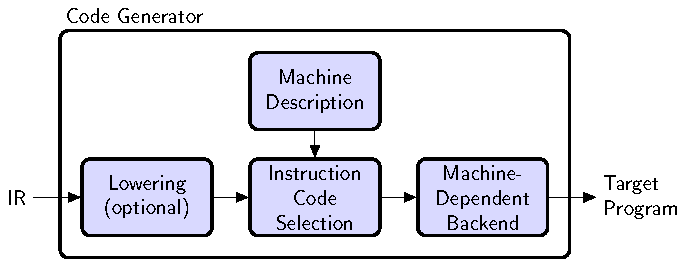
\includegraphics{pgf-fig001}
  \end{center}
  \caption{Scenario: An instruction selector translates a compiler's IR to a
    low-level machine-dependent representation.}
  \label{fig:instruction-selection}
\end{figure}


\begin{algorithm}
\caption{RTL-based code generation scheme.}
\label{alg:rtlisel}
\begin{algorithmic}[1]
\STATE Forward substitution
\STATE Combination of independent effects
\STATE Removal of useless effects
\STATE Validation based on a machine-description
\end{algorithmic}
\end{algorithm}
Code generators in RTL-based compilers are based on the four-step
scheme depicted in Algorithm~\ref{alg:rtlisel}. Forward substitution
forms more complex expressions by substituting sub-expressions with
their defining RTL. Likewise, step (2) combines individual RTLs to a
single expression. After application of these rules, the results are
verified against the machine descriptions. Step (3) simplifies
redundant effects that might result from the application of the
previous steps. RTL expressions that do not represent a native
instruction are discarded in step (4).

The scope of this approach is limited to simple patterns and
constitutes a form of ``poor-man's instruction selection'' achieving
only locally optimal code. Thus, the code quality of RTL-based
compilers such as GCC strongly depends on post-pass RTL-based
optimizations such as common subexpression elimination (CSE) that make
up for missed opportunities.
\subsection{Tree Pattern Matching}
\label{sec:tpm}
Tree pattern matching is more sophisticated than RTL-based instruction
selection, and it is widely used in modern compiler frameworks. The
technique was introduced by Aho and Johnson~\cite{aj:76}. The unit of
translation is a single statement represented in the form of a data
flow tree (DFT). The basic idea is to describe the target instruction
set using an \emph{ambiguous} cost-annotated graph grammar. The
instruction selector seeks for a cost-minimal \emph{cover} of the
DFT. Each of the selected rules have an associated semantic action
that is used to emit the corresponding machine instruction, either by
constructing a new intermediate representation or by rewriting the DFT
bottom-up.
\begin{figure}[ht]
  \begin{center}
%     \begin{tikzpicture}
%       \node at (0,0) [fnode] (rega) {\texttt{VAR:a} };
%       \node at (2,0) [fnode] (regi) {\texttt{VAR:i} };
%       \node at (4,0) [fnode] (cst2) {\texttt{CST:2} };

%       \path (cst2) ++(240:2cm) node[fnode] (shl) {\texttt{SHL} } ;
%       \path (shl) ++(240:1.5cm) node[fnode] (add) {\texttt{ADD} } ;
%       \path (add) ++(270:1.5cm) node[fnode] (ldw) {\texttt{LD} } ;

%       \path[arrow,->] (regi) edge (shl);
%       \path[arrow,->] (cst2) edge (shl);
%       \path[arrow,->,bend left=15] (shl) edge (add);
%       \path[arrow,->,bend right=15] (rega) edge (add);
%       \path[arrow,->] (add) edge (ldw);

%       \node at (-2.8,-2.8) (rega) {
%         \begin{minipage}[]{7cm}
% \begin{verbatim}
% s   <- reg                : 0
% reg <- imm                : 1
% imm <- IMM                : 0
% reg <- VAR                : 0
% reg <- SHL(reg, reg)      : 1
% reg <- SHL(reg, imm)      : 1
% reg <- ADD(reg, reg)      : 1
% reg <- LD(reg)            : 1
% reg <- LD(ADD(reg, reg))  : 1
% reg <- LD(ADD(reg, SHL(reg, imm))) : 1
% \end{verbatim}
%         \end{minipage}
%       };
%     \end{tikzpicture}
    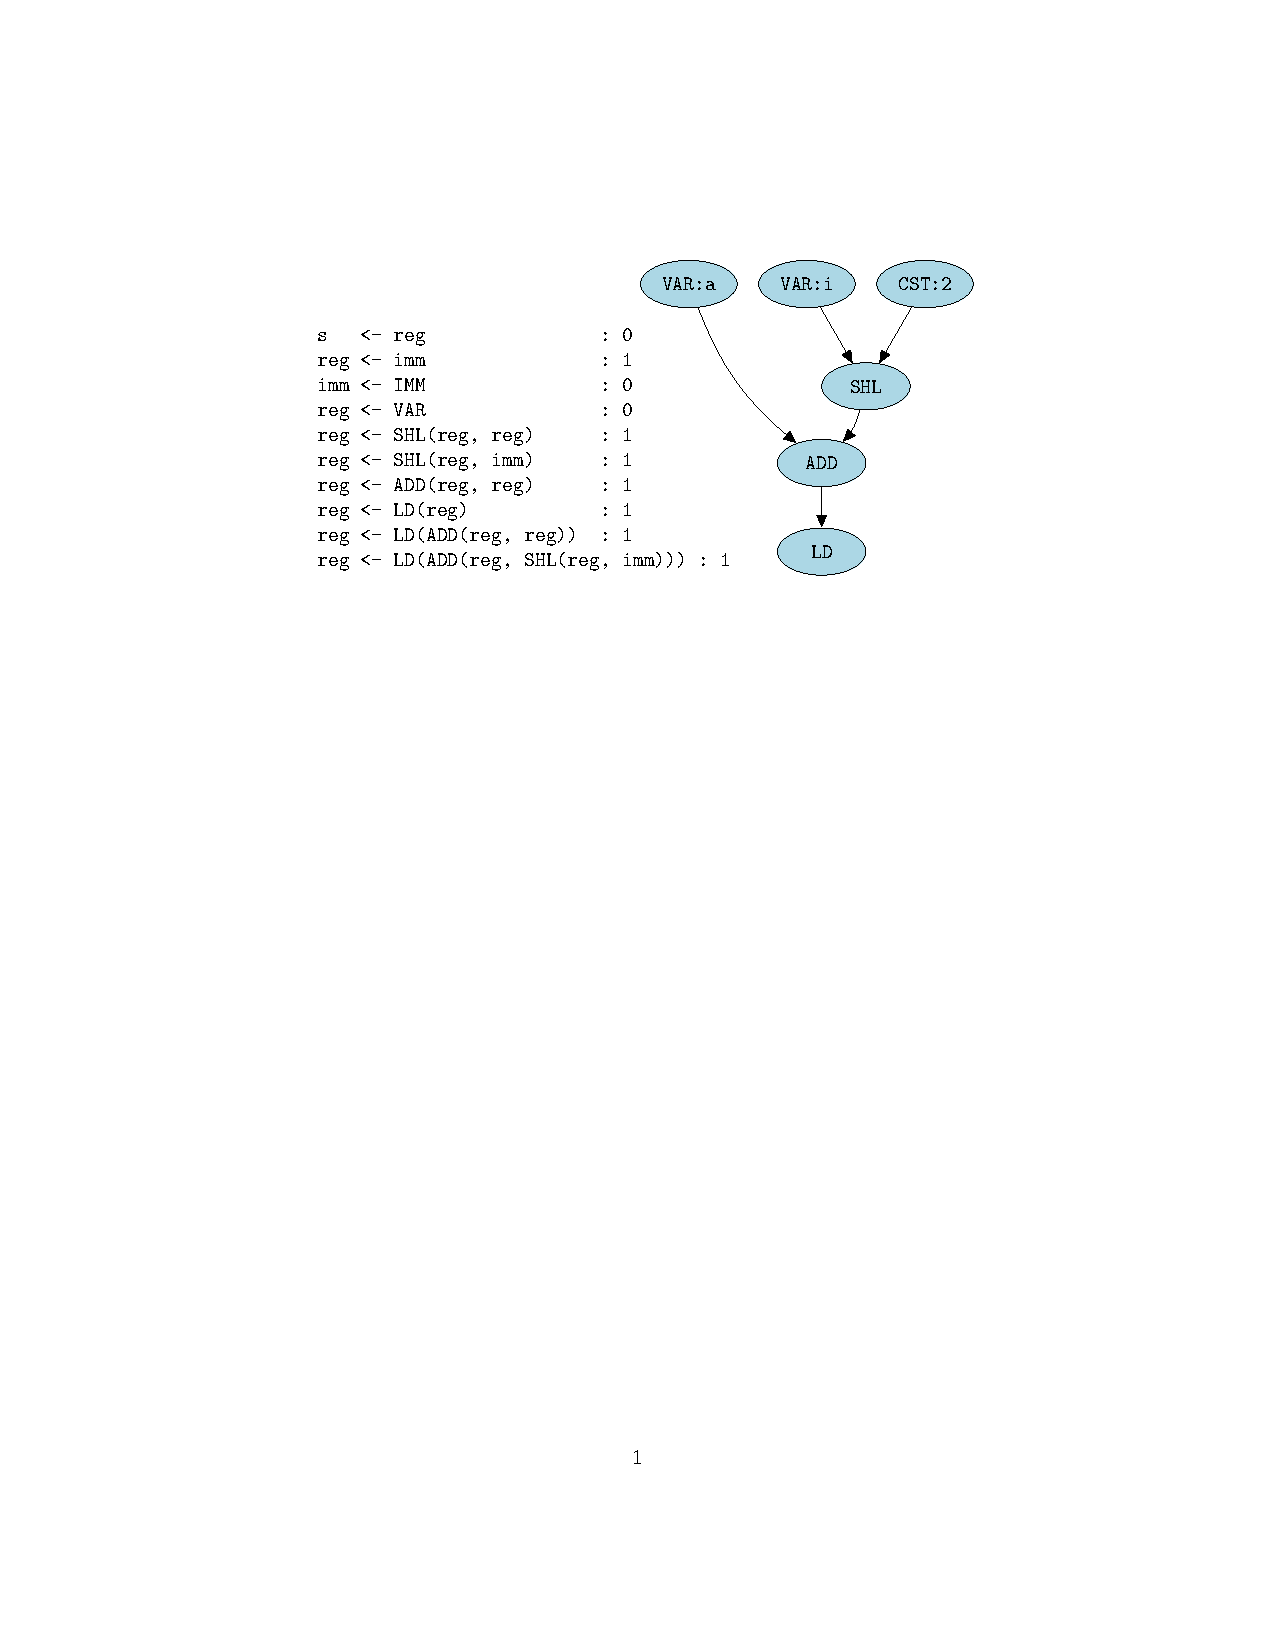
\includegraphics{pgf-fig002}
  \end{center}
  \caption{Example of a data flow tree and a rule fragment with
    associated costs.}\label{fig:tpm}
\end{figure}

An example of a DFT along with a set of rules representing valid ARM
instructions is shown in Figure~\ref{fig:tpm}. Each rule consists of
terminal symbols that are shown in upper-case, and nonterminals that
are shown in lower-case. Terminal symbols match the corresponding
labels of the dataflow trees. Nonterminals are used to chain
individual rules together. Rules that translate from one nonterminal
to another are called \emph{chain rules}. Nonterminal \texttt{s}
denotes a distinguished start symbol. Note that there are multiple
possibilities to obtain a cover of the data-flow tree using the rule
fragment to the left. Each rule has associated costs. The cost of a
tree cover is the sum of the costs of the selected rules.

Aho and Johnson~\cite{aj:76} were the first to propose a dynamic
programming algorithm in order to obtain cost-minimal covers. The
approach of Aho and Johnson was further refined
in~\cite{Balachandran90TreeMatching}, and tree-pattern matching can be
performed in linear time by pre-computing static lookup tables at
compiler compile time. Most implementations rely on the following
two-pass scheme:
\begin{enumerate}
\item[(1)]\emph{labeling:} use dynamic programming in order to
  determine a minimum-cost cover of the given DFT bottom-up.
\item[(2)]\emph{reduce}: traverse the DFT in postfix order and execute
  the semantic actions associated with the chosen rules to obtain a
  semantically equivalent target program.
\end{enumerate}
One of the more popular existing implementations is the tool
\texttt{burg}~\cite{FHP:92} that converts a specification
in the form of a tree grammar into an optimized tree pattern matcher
written in \texttt{C}. While \texttt{burg} computes costs at compiler
compile time and thus requires constant costs,
\texttt{iburg}~\cite{Fraser92Iburg} can handle dynamic costs by
shifting the dynamic programming algorithm to instruction selection
time. This allows the use of dynamic properties for cost computations,
\eg, concrete values of immediates. The additional flexibility is
traded for a small penalty in runtime.  More recent
techniques~\cite{ecg:06} save the computed states for tree nodes in a
lookup table. This approach retains the flexibility of dynamic cost
computations at nearly the speed of precomputed tree parsing automata.

Tree-pattern matching approaches are limited in scope to simple
statements. DAG matching techniques are an approach to overcome these
limitations. However, DAG matching is an NP-complete
problem~\cite{pro98least} in general. A straight forward
generalization~\cite{ertl99optimal} of the algorithm discussed so far
is to treat DAGs as if they were trees and make local choices
irrespective of shared subgraphs. It turns out that this approach is
exact for a specific class of grammars but fails to deliver optimal
solutions in the general case.  For code generation techniques that
exploit aggressively the properties of the target machine, it is
useful to increase the scope of instruction selection further to whole
procedures at a time. An excellent underlying data-structure for code
generation is the SSA graph~\cite{GSW95} that is an extension of DFTs
and represent the data-flow of a procedure in SSA form. In the
following, we will demonstrate how to reduce the instruction selection
problem in SSA graphs to a specialized quadratic assignment problem
(PBQP) \cite{EcksteinKS03}. An extension of \emph{patterns} to
arbitrary acyclic graph structures which we refer to as DAG grammars
is discussed in Section~\ref{sec:dag_patterns} for details. These
extension are useful in the presence of SIMD instructions of CPUs.

As we move from acyclic linear code regions to whole-functions, it
becomes less obvious in which basic block, the selected
machine instructions should be emitted. For chain rules, the obvious
choices are often sub-optimal. We will discuss in
Section~\ref{sec:chain_rule_placement} a polynomial-time algorithm
based on generic network flows that can be applied to generate more
efficient code based on a flexible cost model.

\section{Motivation}
\label{sec:motivation}

\begin{figure}[ht]
  \begin{center}
%     \begin{tikzpicture}
%       \node [anchor=south west] at (-1cm, 1cm) (listing) {
%         \lstset {
%           language=C,
%           basicstyle=\footnotesize,
%           morekeywords={fract_t, _Fract},
%         }
%         \begin{lstlisting}
% typedef unsigned _Fract short fract_t;
% fract_t dot_product(fract_t *p, fract_t *q) {
%   fract_t s = 0, *e = p + N;
%   while(p < e) s += *p++ + *q++;
%   return s;
% }
%        \end{lstlisting}
%       };

%       %tree 1
%       \node [fnode, fill=LightYellow] (vars) {\texttt{VAR:s}};
%       \node [fnode, fill=LightYellow, below of=vars] (cst0) {\texttt{CST:0}};
%       \path[arrow,->] (cst0) -- (vars);

%       %tree 2
%       \node [fnode, fill=LightGreen, below of=cst0] (ret) {\texttt{ret}};
%       \node [fnode, fill=LightGreen, below of=ret] (vars2) {\texttt{VAR:s}};
%       \path[arrow,->] (vars2) -- (ret);

%       %tree 3
%       \node [fnode, fill=LightYellow, right of=vars,
%              node distance=2.8cm] (endp) {\texttt{VAR:e}};
%       \node [fnode, fill=LightYellow, below of=endp] (add) {\texttt{ADD}};
%       \node [fnode, fill=LightYellow] (varp) at ($(add)+(-1cm, -1.5cm)$) {\texttt{VAR:p}};
%       \node [fnode, fill=LightYellow] (cstn) at ($(add)+(+1cm, -1.5cm)$){\texttt{CST:2N}};
%       \path[arrow,->] (add) -- (endp);
%       \path[arrow,->] (varp) -- (add);
%       \path[arrow,->] (cstn) -- (add);

%       %tree 4
%       \node [fnode] at (10.5, 3cm) (vars3) {\texttt{VAR:s}};
%       \node [fnode] at ($(vars3)+(-3cm,-1.5cm)$) (add2) {\texttt{ADD}};
%       \node [fnode, below of=add2] (mul) {\texttt{MUL}};
%       \node [fnode, below of=vars3, node distance=3cm] (vars4) {\texttt{VAR:s}};

%       \node [fnode] at ($(mul)+(3cm,-1.5cm)$) (ldq) {\texttt{LD}};
%       \node [fnode, below of=ldq, node distance=3cm] (varq) {\texttt{VAR:q}};
%       \node [fnode, left of=ldq, node distance=1.6cm] (varq2) {\texttt{VAR:q}};
%       \node [fnode] at ($(ldq)+(-1cm,-1.5cm)$) (inc) {\texttt{INC}};
%       \path[arrow,->, bend left=5] (inc) edge (varq2);
%       \path[arrow,->, bend left=5] (varq) edge (inc);
%       \path[arrow,->, bend right=15] (varq) edge (ldq);

%       \node [fnode] at ($(ldq)+(-3.9cm,0cm)$) (ldp) {\texttt{LD}};
%       \node [fnode, below of=ldp, node distance=3cm] (varp) {\texttt{VAR:p}};
%       \node [fnode, left of=ldp, node distance=1.6cm] (varp2) {\texttt{VAR:p}};
%       \node [fnode] at ($(ldp)+(-1cm,-1.5cm)$) (inc2) {\texttt{INC}};
%       \node [fnode] at ($(varp)+(1.7cm,0cm)$) (vare) {\texttt{VAR:e}};
%       \node [fnode] at ($(inc2)+(2.2cm,0cm)$) (lt) {\texttt{<}};
%       \path[arrow,->, bend left=5] (inc2) edge (varp2);
%       \path[arrow,->, bend left=5] (varp) edge (inc2);
%       \path[arrow,->, bend right=15] (varp) edge (ldp);
%       \path[arrow,->, bend left=5] (varp) edge (lt);
%       \path[arrow,->, bend right=5] (vare) edge (lt);

%       \path[arrow,->, bend left=5] (ldp) edge (mul);
%       \path[arrow,->, bend right=15] (ldq) edge (mul);
%       \path[arrow,->] (mul) edge (add2);
%       \path[arrow,->, bend right=15] (vars4) edge (add2);
%       \path[arrow,->, bend left=15] (add2) edge (vars3);
%     \end{tikzpicture}
    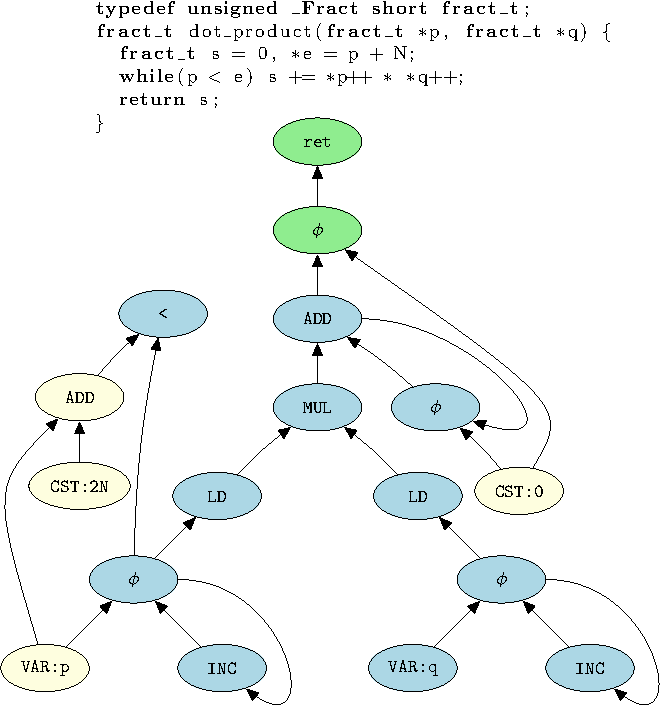
\includegraphics{pgf-fig003}
  \end{center}
  \caption{Instruction selection DAGs for a vector dot-product in
    fixed-point artithmetic.}\label{fig:dot_product}
\end{figure}

We demonstrate that DAG based instruction selection is not
sufficient to generate optimal code as shown in
Figure~\ref{fig:dot_product}. For the example we assume an ARM-like RISC
architecture. The code implements a simple vector dot-product using
fixed-point arithmetic in Embedded~C. The color of DAG nodes depicts
the particular basic block they belong to, and we assume the notion of type
annotation to distinguish fixed-point data types from
regular integer arithmetic.

For sake of simplicity, we neglect the details including numerical precision,
loop control code, and we disregard output- and anti-dependencies
that have to be respected in order to maintain semantic equivalence.
For example, we have to emit the
post-increment for variables \texttt{p} and \texttt{q} \emph{after} the
corresponding loads which is neglected.

In our grammar fixed-point values are represented by
nonterminal symbol \texttt{fp} and the cost function
separates fixed-point arithmetic from general integer arithmetic,
\ie, we alter the grammar introduced in Figure~\ref{fig:tpm} as
shown below:
\begin{alltt}
   reg <- VAR : is\_fixed_point() ? \(\infty\) : 0
   fp  <- VAR : is\_fixed_point() ? 0 : \(\infty\)
\end{alltt}
For fixed-point values most arithmetic and bitwise operations are
identical to their integer equivalents. However, some operations have
a different semantics, \eg, multiplying two fixed-point values in
format $m.i$ results in a value with $2i$ digits of fraction. The
result of the multiplication has to be adjusted by a shift operation
to the right. The adjustment can be modeled for an ARM-like
architecture by following rule fragment that models double-precision
fixed-point values with nonterminal \texttt{fp2}:
\begin{alltt}
   fp2 <- MUL(fp, fp)   : 1   \{ MUL Rd, Rm, Rs \}
   fp  <- fp2           : 1   \{ LSR Rd, Rm, i  \}
   fp  <- ADD(fp, fp)   : 1   \{ ADD Rd, Rm, Rs \}
   fp2 <- ADD(fp2, fp2) : 1   \{ ADD Rd, Rm, Rs \}
\end{alltt}
We can perform the accumulation for double-precision fixed
point values at the same cost as for \texttt{fp}. Thus, it would be
beneficial to move the necessary shift from the inner loop to the
return block, performing the intermediate calculations in the extended
format. However, as a DAG based matcher processes basic block by
basic block, the information of having values as double-precision
cannot be hoisted across basic block boundaries.

To overcome this limitation, we can extend the scope of the matching
algorithm to the computational flow of a whole procedure. SSA graphs
provide a very suitable vehicle for performing instruction selection for
manifold reasons:  First, in
contrast to classical tree or DAG representations, SSA graphs enable
the matching of circular flow stemming from program loops.
Second, SSA graphs often arise naturally in modern
compilers as intermediate code is already in SSA form. Third, the
set of edges fully specifies the set of data dependencies that have to
be respected as there are no additional output or
anti-dependencies. These additional dependencies significantly
complicate or limit DAG based techniques.

\begin{figure}
  \begin{center}
%     \begin{tikzpicture}

%       \node [fnode, fill=LightGreen] (ret) {\texttt{ret}};
%       \node [fnode, fill=LightGreen, below of=ret] (phi1) {$\phi$};
%       \node [fnode, below of=phi1] (add1) {\texttt{ADD}};
%       \node [fnode, below of=add1] (mul) {\texttt{MUL}};
%       \node [fnode, right of=mul, node distance=2cm] (phi3) {$\phi$};
%       \node [fnode, fill=LightYellow, below right of=phi3, node distance=2cm]
%             (cst0) {\texttt{CST:0}};
%       \path[arrow,->] (mul) edge (add1);
%       \path[arrow,->] (add1) edge (phi1);
%       \path[arrow,->] (phi1) edge (ret);

%       \node [fnode] at ($(mul)+(-1.7cm,-1.5cm)$) (ldp) {\texttt{LD}};
%       \node [fnode, below left of=ldp, node distance=2cm] (phip) {$\phi$};
%       \node [fnode, fill=LightYellow] at ($(phip)+(-1.5cm,-1.5cm)$) (varp) {\texttt{VAR:p}};
%       \node [fnode] at ($(phip)+(+1.5cm,-1.5cm)$) (inc) {\texttt{INC}};
%       \path[arrow,->] (varp) -- (phip);
%       \path[arrow,->] (inc) -- (phip);
%       \path[arrow,->] (phip) -- (ldp);
%       \path[arrow,->, bend left=5] (ldp) edge (mul);
%       \path [arrow,->] (phip) .. controls ($(phip.east)+(2cm,0cm)$)
%             and ($(inc.east)+(1cm,-1.5cm)$) .. (inc);

%       \node [fnode] at ($(mul)+(1.7cm,-1.5cm)$) (ldq) {\texttt{LD}};
%       \node [fnode, below right of=ldq, node distance=2cm] (phiq) {$\phi$};
%       \node [fnode] at ($(phiq)+(-1.5cm,-1.5cm)$) (varq) {\texttt{VAR:q}};
%       \node [fnode] at ($(phiq)+(+1.5cm,-1.5cm)$) (inc) {\texttt{INC}};
%       \path[arrow,->] (varq) -- (phiq);
%       \path[arrow,->] (inc) -- (phiq);
%       \path[arrow,->] (phiq) -- (ldq);
%       \path[arrow,->, bend right=5] (ldq) edge (mul);
%       \path [arrow,->] (phiq) .. controls ($(phiq.east)+(2cm,0cm)$)
%             and ($(inc.east)+(1cm,-1.5cm)$) .. (inc);

%       \node [fnode] at ($(phip)+(0.5cm,4.5cm)$) (lt) {\texttt{<}};
%       \node [fnode, fill=LightYellow, below left of=lt,
%              node distance=2cm] (add) {\texttt{ADD}};
%       \node [fnode, fill=LightYellow, below of=add] (cstn) {\texttt{CST:2N}};
%       \path[arrow,->, bend left=5] (add) edge (lt);
%       \path[arrow,->] (varp) ..controls ($(cstn)+(-1.5cm,0)$) .. (add);
%       \path[arrow,->] (cstn) -- (add);
%       \path[arrow,->, bend left=5] (phip) edge (lt);
%       \path[arrow,->, bend right=5] (phi3) edge (add1);
%       \path[arrow,->] (add1) .. controls ($(add1.east)+(2cm,0cm)$)
%             and ($(phi3.east)+(2cm,-1cm)$) .. (phi3);
%       \path[arrow,->] (cst0) .. controls ($(phi3.east)+(1.5cm,0cm)$) ..  (phi1);
%       \path[arrow,->,bend right=5] (cst0) edge (phi3);

%     \end{tikzpicture}
    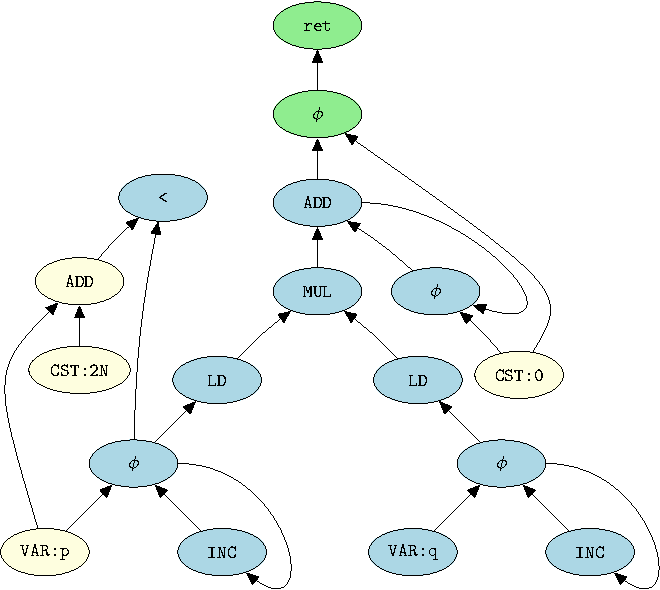
\includegraphics{pgf-fig004}
  \end{center}
  \caption{Corresponding SSA graph for the example introduced in
    Figure~\ref{fig:dot_product}.}\label{fig:ssa_graph}
\end{figure}

The corresponding SSA graph for the example introduced in
Figure~\ref{fig:dot_product} is shown in Figure~\ref{fig:ssa_graph}.
Nodes in the SSA graph represent a single operation while edges
describe a flow of data that is produced at the source node and that
is consumed at the target node. Incoming edges have an order which reflects the argument
order of the operation. In the figure the color of the nodes
show to which basic block the operations belong to. An instruction
selector operating on the SSA graph is free to propagate nonterminal \texttt{fp2}
across the $\phi$ node prior to the return and emits the
code for the shift to the right in the return block.

As SSA graphs are potentially cyclic, no dynamic
programming approach can be employed for instruction selection. To get
a handle on code selection for SSA graphs, we will discuss in the following
an approach based on a reduction to a quadratic mathematical programming
problem (PBQP) \cite{EcksteinKS03,1269857,Ebner08} that has been adopted
by at least two major embedded system compiler vendors. We continue with a short
introduction to PBQP before discussing the main problem formulation
and two extensions that allow for more flexible grammars and optimal
chain code placement.

\section{Partitioned Boolean Quadratic Programming}
% \emph{2 pages}; introduction into PBQP, algorithms, and applications
Partitioned Boolean Quadratic Programming
(PBQP) is a generalized quadratic assignment problem that has proven
to be effective for a wide range of applications in embedded code
generation, \eg, instruction selection, register assignment, address
mode selection \cite{Eck03}, or bank selection for architectures with
partitioned memory \cite{journals/tecs/ScholzBX08}. Instead of
problem-specific algorithms, these problems can be modeled in terms of
generic {PBQP}s that are solved using a common solver library. PBQP
is flexible enough to model irregularities of embedded architectures
that are hard to cope with using traditional heuristic approaches.

\subsection{Problem Definition}
A PBQP is a generalized quadratic assignment problem proposed by
Scholz and Eckstein for various sub-problems of embedded code
generation~\cite{ScholzE02,Eck03}. Consider a set of discrete
variables $X=\{x_1,\ldots,x_n\}$ and their finite domains
$\{\vardomain_1,\ldots,\vardomain_n\}$. A solution of PBQP is a
mapping $h$ of each variable to an element in its domain. The quality of a
solution is based on the contribution of two sets of terms,
\begin{enumerate}
\item for assigning variable $x_i$ to the element $d_i$ in
  $\vardomain_i$. The quality of the assignment is measured by a
  \emph{local cost function} $c(x_i, d_i)$,
\item for assigning two related variables $x_i$ and $x_j$ to the
  elements $d_i \in \vardomain_i$ and $d_j \in \vardomain_j$.  We
  measure the quality of the assignment with a \emph{related cost
    function\/} $C(x_i,x_j, d_i,d_j)$,
\end{enumerate}
and the total cost of a solution $h$ is given as,
\begin{equation}
  f\! =\! \sum_{1 \leq i \leq n} \hspace{-1mm} c(x_i,h(x_i)) + \hspace{-3mm} \sum_{1 \leq i < j  \leq n} \hspace{-3.5mm}
  C\left (x_i,x_j, h(x_i), h(x_j) \right). \label{eqn-pbqp}
\end{equation}
The PBQP problem seeks for an assignment with minimum total costs.

We can alternatively formulate PBQP using matrix calculus: a discrete
variable $x_i$ is represented as a boolean vector $\vec{x_i}$ whose
elements are zeros and ones and whose length is determined by the
number of elements in its domain $|\vardomain_i|$. Each 0-1 element of
$\vec{x_i}$ corresponds to an element of $\vardomain_i$. An assignment
of $x_i$ to $d_i$ is represented as a unit vector whose element for
$d_i$ is set to one. Hence, a valid assignment for a variable $x_i$ is
modeled by the constraint $\vec{x_i}^T \vec{1}=1$ that restricts
vectors $\vec{x_i}$ such that exactly one vector element is assigned
one; all other elements are set to zero.

The related cost function $C(x_i,x_j,d_i,d_j)$ is decomposed for each
pair $(x_i,x_j)$. The costs for the pair are represented as matrix
${\matrixfont C}_{ij}$. A matrix element corresponds to an assignment
$(d_i, d_j)$. Similarly, the local cost function $c(x_i,d_i)$ is
mapped to cost vectors $\vec{c_i}$. We can formulate a PBQP as the
following mathematical program:
\begin{align}
  \min f(X) &=
  \sum_{1 \leq i \leq n} \vec{x_i}^{T} \vec{c_i}  +
  \sum_{1 \leq i < j \leq n}
  \vec{x_i}^{T}  {\matrixfont C}_{ij} \vec{x_j} \\
  \ s.t. \,        &\,  \forall 1 \leq i \leq n : \vec{x_i} \in \{0,1\}^{|\vardomain_i|}  \label{def:constraints1}\\
  &\,  \forall 1 \leq i \leq n : \vec{x_i}^T \vec{1} = 1 \label{def:constraints2}
\end{align}
A solution satisfying Constraints~\ref{def:constraints1} and
~\ref{def:constraints2} maps each boolean decision vector $\vec{x_i}$
to a binary vector that contains a single one element. This defines a
one-to-one mapping among decision vectors $\vec{x_i}$ and elements in
their domain $\vardomain_i$. Thus, the domain for the objective
function is the cross product of the domains for the individual
variables $\vardomain_1 \times \dots \times \vardomain_n$. The
solution to a PBQP is not necessarily unique, \ie, there are in
general multiple solution vectors $\bar{X}$ with the same minimal
objective value.

A PBQP problem has an underlying graph structure graph $G=(V,E,C,c)$,
which we refer to as a PBQP graph. For each decision vector
$\vec{x_i}$ we have a corresponding node $v_i \in V$ in the graph, and
for each cost matrix ${\matrixfont C}_{i,j}$ that is not the zero
matrix, we introduce an edge $e=(v_i,v_j)$. The cost functions $c$ and
$C$ map nodes and edges to the original cost vectors and matrices
respectively. Note, that due to the properties of quadratic forms,
there is an implicit reverse edge $e'=(v_j,v_i)$ for each edge
$e=(v_i,v_n)$ and $C(e) = C(e')^T$. A PBQP graph is free of self- and
multi-edges. We will present an example later in this chapter in the
context of instruction selection.

In general, finding a solution to this minimization problem is NP
hard.  However, for many practical cases, the PBQP instances are
sparse, \ie, many of the cost matrices ${\matrixfont C}_{i,j}$ are
zero matrices and do not contribute to the overall solution. Thus,
optimal or near-optimal solutions can often be found within reasonable
time limits.
We will discuss two algorithmic approaches for PBQP that have been
proven to be efficient in practice for instruction selection problems,
\ie, a polynomial-time heuristic algorithm and a branch-\&-bound based
algorithm with exponential worst case complexity.

\subsection{Heuristic Algorithm}
\label{sec:pbqp:heuristic}
In this section, we introduce an algorithm for PBQP proposed by
Scholz and Eckstein \cite{ScholzE02,Eck03}.  For a certain subclass of
PBQP, their algorithm produces provably optimal solutions in time
${\cal O}(n m^3)$, where $n$ is the number of discrete variables and
$m$ is the maximal number of elements in their domains, \ie, $m=\max
\left(|\vardomain_1|,\ldots,|\vardomain_n\right|)$. For general
{PBQP}s, however, the solution may be sub-optimal.

\begin{algorithm}
\caption{PBQP Heuristic}
\label{alg:pbqp:heuristic}
\begin{algorithmic}
  \STATE \COMMENT{\textbf{\emph{Phase I: reduction}}}
  \WHILE{$\exists v \in V : \deg v > 0$}
  \STATE choose vertex $v \in V: 0 < \deg (v) \leq \deg (v') \ \forall v'
  \in V : \deg(v') > 0$
  \IF{$\deg(v) == 1$}
  \STATE \textbf{RI}(v)
  \ELSIF{$\deg(v) == 2$}
  \STATE \textbf{RII}(v)
  \ELSE
  \STATE \textbf{RN}(v) \COMMENT{solution may be sub-optimal if RN is applied}
  \ENDIF
  \STATE remove $v$ from the graph
  \ENDWHILE
  \STATE
  \STATE \COMMENT{\textbf{\emph{Phase II: trivial solution}}}
  \FORALL{$v_i \in V$}
  \STATE determine solution for $v_i$ by finding the minimum element
  in $c_i$
  \ENDFOR
  \STATE
  \STATE \COMMENT{\textbf{\emph{Phase III: back-propagation}}}
  \STATE re-insert the remaining nodes in reversed elimination order
  until a solution for the original graph is obtained
\end{algorithmic}
\end{algorithm}
The algorithm works in three phases as shown in
Algorithm~\ref{alg:pbqp:heuristic}. First, the PBQP graph is reduced
until only nodes of degree $0$ are left. For these nodes, a solution
can easily be found using a local minimum computation. In a last step,
the eliminated nodes are re-inserted in reversed order thereby
computing a solution for the original problem instance.

\subsubsection{Phase I: Reduction.} Eliminating nodes from the PBQP graph
is equivalent to the elimination of decision vectors from the original
problem. The algorithm removes nodes from the graph until only nodes
of degree $0$ remain. Nodes to be removed are chosen according to
their degree in increasing order. In practice, this can be
accomplished efficiently by putting nodes into buckets according to
their degree. The algorithm selects a node from the bucket with the
smallest index that is non-empty.

Nodes with degree one or two can be eliminated without loss of
optimality using reductions RI and RII respectively. If the algorithm
reaches a point where only nodes with degree three or more are left,
the problem becomes irreducible and a heuristic is applied, which is
called RN. The heuristic chooses a beneficial discrete variable and a
good assignment for it by searching for local minima. The obtained
solution is guaranteed to be optimal if the reduction RN is not
used~\cite{Eck03}.

\paragraph{RI Reduction.}
Let $v_i$ be a node with degree one and let $v_j$ denote its only
adjacent vertex in the PBQP graph, we can eliminate $v_i$ and the
incident edge $(v_i, v_j)$ simply by removing them from the PBQP
graph. The cost vector associated with $v_j$ is incremented by the
minimum costs over all possible choices of $v_i$. More formally, the
updated cost vector $\vec{c_j}'$ is given by
$$\vec{c_j}'(a) = \vec{c_j}(a) + \min({\matrixfont C}_{j,i}(a,:) +
\vec{c_i}).$$ As for the reduction RII, it is easy to show that the
optimal objective value for the modified graph corresponds to the
optimal value of the original problem. A formal proof is given by
Eckstein \cite{Eck03}.

\paragraph{RII Reduction.}
Reduction RII follows the same idea as reduction RI. The operation is
applied to nodes $v_i$ with degree two. The two adjacent nodes are
denoted by $v_j$ and $v_k$ respectively. Vertex $v_i$ is removed and
the minimal costs for $v_i$ depending on choices for $v_j$ and $v_k$
are added to the cost matrix ${\matrixfont C}_{j,k}$. The new cost
matrix ${\matrixfont C}'_{j,k}$ is defined as follows:
$${\matrixfont C}'_{j,k}(a,b) = {\matrixfont C}_{j,k}(a,b) +
\min({\matrixfont C}_{j,i}(a,:) + {\matrixfont C}_{k,i}(b,:) + \vec{c_i}.$$

\paragraph{RN Reduction.}
PBQP graphs that cannot be reduced using reductions RI and RII are
called \emph{irreducible}. The smallest example for an irreducible
graph is the complete graph with four nodes $K_4$. One possibility to
deal with irreducible graphs is recursive enumeration. However,
recursive enumeration has exponential worst-case complexity which
makes it an infeasible approach for most applications. Instead, a
heuristic called RN is applied that reduces a node using a local
minimum computation. The basic idea is to make a decision as if the
node and the adjacent vertices are disconnected from the rest of the
PBQP graph. While reductions RI and RII can be shown to maintain the
optimality of the obtained solution, RN does not and leads to
sub-optimal solutions in general. Let $v_i$ denote a vertex of degree
three or more, we heuristically select the index with minimal costs
from the cost vector $\vec{c}'$ defined as follows:
$$\vec{c}'(a) = \vec{c_i}(a) + \sum_{(v_i,v_j) \in E}{\min({\matrixfont C}_{i,j}(a,:)
  + \vec{c_j})}.$$ Let $s_i$ denote such an index with minimal costs
in $\vec{c}'$, it remains to update the cost vectors for adjacent
nodes accordingly. For each adjacent node $v_j$, the new modified cost
vector $\vec{c_j}'$ evaluates to $\vec{c_j}' = \vec{c_j} +
{\matrixfont C}_{i,j}(s_i,:)$.

\subsubsection{Phase II: Trivial Solution.}
Upon completion of the reduction phase, there are only nodes with
degree $0$ left in the PBQP graph. This corresponds to a PBQP in
matrix notation where all cost matrices are the zero matrix and the
cost function is reduced to $$\min f(X) = \sum_{1 \leq i \leq n}
\vec{x_i}^{T} \vec{c_i}.$$ Since there are no dependencies among the
decision variables, the minimization problem is equivalent to the
evaluation of the term $$\sum_{1 \leq i \leq n} \min
_{x_i}\vec{x_i}^{T} \vec{c_i}.$$ Thus, we can determine the solution
for each decision variable $x_i$ by finding the smallest element in
its associated cost vector $c_i$.

\subsubsection{Phase III: Back-Propagation.}
\begin{algorithm}
\caption{Back-Propagation}
\label{alg:pbqp:back-propagation}
\begin{algorithmic}
  \FORALL{$v_i \in V$}
  \STATE $s_{v_i} = k : c_i(k) = \min(c_i)$
  \ENDFOR
  \WHILE{$S$ not empty}
  \STATE pop node $v_i$ from S
  \STATE $\vec{c} = \vec{c_i}$
  \FORALL{$(v_j,v_i) \in E$}
  \STATE $\vec{c} += {\matrixfont C}_{j,i}(s_{v_j},:)$
  \ENDFOR
  \STATE $s_{v_i} = k : c(k) = \min(c)$
  \ENDWHILE
\end{algorithmic}
\end{algorithm}
In the back-propagation phase, nodes are re-inserted in reversed
elimination order. At each step, the solution for the newly inserted
node can be easily determined as the decision vectors for adjacent
nodes are already known; see \cite{Eck03} for a formal proof. The
algorithm for a PBQP graph $G=(V,E,C,c)$ is shown in pseudo-code in
Algorithm~\ref{alg:pbqp:back-propagation}. We denote with $S$ the
stack of eliminated nodes from Phase I.

\subsection{Branch~\&~Bound}
\label{sec:pbqp:bab}
Branch~\&~Bound (BAB) is a very generic and efficient enumeration
scheme for combinatorial optimization problems that has been
successfully applied to a large set of NP hard optimization problems,
\eg, integer programming, knapsack problem, traveling salesman
problem, or maximum satisfiability problem.

The main idea is to arrange the search space such that large parts can
be explored only implicitly. At any point in the optimization process,
we maintain a pool of yet unexplored subspaces together with the best
solution found so far. Initially, there is only one subset
representing the whole solution space and the best solution is set to
$\infty$\footnote{Without loss of generality, we assume minimization
  problems within this chapter.}. Subspaces are created dynamically
and arranged in a so-called search tree. The key-idea is that large
portions of these subspaces can be eliminated by comparing their lower
bounds with the best solution found so far.

Any BAB algorithm consists of the following key ingredients:
\begin{enumerate}
\item \emph{Bounding procedure:} for a given subspace of the solution
  space, compute a \emph{tight} lower bound on the best solution value
  that is obtainable within this subspace.
\item \emph{Selection strategy:} select the next live subproblem to be
  investigated in the search procedure. Popular techniques are breath
  first search (BFS), depth first search (DFS), and best first
  search. The latter always selects the subproblem with the lowest
  bound among the set of live subproblems. An experimental evaluation
  of the various strategies for QAP can be found in \cite{ClausenP99}.
\item \emph{Branching rule:} divide the considered subspace into two
  or more subspaces to be considered in subsequent iterations of the
  algorithm.
\end{enumerate}

An advantage of BAB based algorithms that becomes more and more
important with the rise of multi- and many-core systems is their
ability to scale naturally with the number of cores.

\begin{figure}
  \begin{center}
%     \begin{tikzpicture}
%       \tikzstyle{fbox} = [rectangle, draw, sharp corners, text
%       width=2cm,minimum width=2cm, minimum height=1cm,text badly centered,
%       node distance=3cm, inner sep=2pt, fill=LightBlue]

%       \node at (0,0)     [fbox] (v1) {P};
%       \node at (-2,-2) [fbox] (v2) {$x_{i_1} = (1, 0,\dots,0)$};
%       \node at (0,-2)  [] (v3) {$\dots$};
%       \node at (2,-2)  [fbox] (v4) {$x_{i_1} = (0, 0,\dots,1)$};

%       \node at (-4,-4)   [fbox] (v5) {$x_{i_2} = (1, 0,\dots,0)$};
%       \node at (-2,-4)   [] (v6) {$\dots$};
%       \node at (0,-4)    [fbox] (v7) {$x_{i_2} = (0, 0,\dots,1)$};

%       \path [arrow,->] (v1) -- (v2);
%       \path [arrow,->] (v1) -- (v4);
%       \path [arrow,->] (v2) -- (v5);
%       \path [arrow,->] (v2) -- (v7);
%     \end{tikzpicture}
    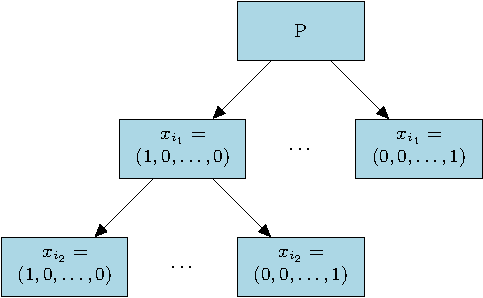
\includegraphics{pgf-fig005}
  \end{center}
  \caption{A fragment of the search tree for a BAB based PBQP algorithm.}
  \label{fig:pbqp:bab-tree}
\end{figure}

PBQP allows for a natural mapping to the BAB scheme outline so far
\cite{DBLP:conf/jmlc/HamesS06}. As in
Section~\ref{sec:pbqp:heuristic}, reductions RI and RII can be applied
until a irreducible graph remains. A subspace of the solution space is
represented by a node in a search tree as shown in
Figure~\ref{fig:pbqp:bab-tree}. A subspace is divided into smaller
subspaces by selecting a yet unconsidered decision vector $x_i$ from
one of the leaf nodes and creating $|\vardomain_i|$ child nodes, each
of which representing one of the possible assignments for $x_i$. The
whole set of partial assignments for a subspace of the solution space
can be obtained by walking the search tree back to the root node.

A simple lower bound $f_l$ on the objective function can be obtained
using the following term:
$$f_l = \sum_{1 \leq i \leq n} \min c_i + \sum_{1 \leq i < j  \leq n}
\min {\matrixfont C}_{i,j}.$$ For inner nodes on the search tree, some
of the variables $x_i$ are already included in the partial assignment
and evaluate to constants that replace the minimum computation and
lead to tighter bounds in general. Note that we can derive the new
lower bound after a branching operation in an incremental way using
the lower bound of the parent node.

Leaf nodes that are not yet solved are called \emph{live} and usually
kept in a priority queue according to their lower
bound. Various selection strategies are possible. The
\emph{best first search} strategy leads to good results in practice
for instruction selection problems.

A whole subspace can be pruned from the search if its lower bound
exceeds a global upper bound on the value of the optimal
solution. Initially, the global upper bound can be set to
$\infty$. However, faster convergence can be achieved in general by
applying a heuristic algorithm such as the method proposed in
Section~\ref{sec:pbqp:heuristic} in a pre-processing step. This will
allow the BAB algorithm to prune large subspaces early in the
optimization process.

\section{Code Selection for Tree Patterns}
% \emph{5 pages}; modeling, continued example
The matching problem for SSA graphs reduces to PBQP
\cite{EcksteinKS03} in a straightforward fashion. In the basic
modeling, SSA and PBQP graphs coincide. This means that the number of
decision vectors and cost matrices in the PBQP is determined by the
number of nodes and edges in the SSA graph respectively. A solution
for the PBQP instance induces a complete cost minimal cover of the SSA
graph.

As in traditional tree pattern matching, an ambiguous graph grammar
consisting of tree patterns with associated costs and semantic actions
is used. Input grammars have to be \emph{normalized}. This means that
each rule is either a \emph{base rule} or a \emph{chain rule}. A
base rule is a production of the form $\texttt{nt}_0 \leftarrow
\textit{op} ( \texttt{nt}_1, \dots, \texttt{nt}_{k_p} )$ where
$\texttt{nt}_i$ are non-terminals and $\textit{op}$ is a terminal
symbol, \ie, an operation represented by a node in the SSA graph. A
chain-rule is a production of the form $\texttt{nt}_0 \leftarrow
\texttt{nt}_1$, where $\texttt{nt}_0$ and $\texttt{nt}_1$ are
non-terminals.  A production rule $\texttt{nt} \leftarrow
\textit{op}_1 ( \alpha, \textit{op}_2 (\beta), \gamma))$ can be
normalized by rewriting the rule into two production rules
$\texttt{nt} \leftarrow \textit{op}_1 ( \alpha, \texttt{nt}' ,
\gamma)$ and $\texttt{nt}' \leftarrow \textit{op}_2 ( \beta)$ where
$\texttt{nt}'$ is a new non-terminal symbol and $\alpha,\beta$ and
$\gamma$ denote arbitrary pattern fragments.  This transformation can
be iteratively applied until all production rules are either chain
rules or base rules.

\begin{figure}
  \begin{center}
%     \begin{tikzpicture}
%       \tikzstyle{arrow} = [draw,>=triangle 45]
%       \tikzstyle{tarrow} = [arrow,thick]

%       \path (275:11cm) node[draw,shape=rectangle,fill=LightBlue]
%       {
%         \begin{minipage}{5.2cm}
%           \small
%           \begin{tabular}{l|l}
%             $R_1$ & \texttt{{imm} <- IMM}\\
%             $R_2$ & \texttt{reg <- VAR}\\
%             $R_3$ & \texttt{reg <- imm}\\
%             $R_4$ & \texttt{reg <- SHL(reg, {reg})}\\
%             $R_5$ & \texttt{reg <- SHL(reg, imm)}\\
%             $R_6$ & \texttt{t1 \ <- SHL(reg, imm)}\\
%             $R_7$ & \texttt{reg <- ADD(reg, reg)}\\
%             $R_8$ & \texttt{t2 \ <- ADD(reg, t1)}\\
%             $R_9$ & \texttt{t3 \ <- ADD(reg, reg)}\\
%             $R_{10}$ & \texttt{reg <- LDW(reg)}\\
%             $R_{11}$ & \texttt{reg <- LDW(t2)}\\
%             $R_{12}$ & \texttt{reg <- LDW(t3)}
%           \end{tabular}
%         \end{minipage}
%       }
%       ;

%       \tikzstyle{every node}=[minimum size=1.3cm];

%       \path (0:0) node[draw,shape=circle,fill=LightBlue]
%       (rega) {\small\texttt{VAR:a} }
%       node[right=14pt] {
%         \small
%         $\begin{array}{ccc}
%           & \color{OrangeRed}R_2 &  \\ \cline{2-2}
%           ( & \color{OrangeRed}0 & )
%         \end{array}$
%       }
%       node[right=3cm,draw,shape=circle,fill=LightBlue] (regi) {\small\texttt{VAR:i}}
%       node[right=4.3cm] {
%         \small
%         $\begin{array}{ccc}
%           & \color{OrangeRed}R_2 &  \\ \cline{2-2}
%           ( & \color{OrangeRed}0 & )
%         \end{array}$
%       }
%       node[right=8cm,draw,shape=circle,fill=LightBlue] (cst2) {\small\texttt{CST:2}}
%       node[right=9.3cm] {
%         \small
%         $\begin{array}{ccc}
%           & \color{OrangeRed}R_1 &  \\ \cline{2-2}
%           ( & \color{OrangeRed}0 & )
%         \end{array}$
%       };

%       \path (cst2) ++(250:4cm) node[draw,shape=circle,fill=LightBlue]
%       (shl) {\small\texttt{SHL} }
%       node[right=14pt] {
%         \small
%         $\begin{array}{ccccc}
%           & R_4 & R_5 & \color{OrangeRed}R_6 & \\ \cline{2-4}
%           ( & 1 & 1 & \color{OrangeRed}0 & )
%         \end{array}$
%       };

%       \path (shl) ++(250:5cm) node[draw,shape=circle,fill=LightBlue]
%       (add) {\small\texttt{ADD} }
%       node[right=14pt] {
%         \small
%         $\begin{array}{ccccc}
%           & R_7 & \color{OrangeRed}R_8 &  R_9 & \\ \cline{2-4}
%           ( & 1 & \color{OrangeRed}0 & 0 & )
%         \end{array}$
%       };

%       \path (add) ++(270:4cm) node[draw,shape=circle,fill=LightBlue]
%       (ldw) {\small\texttt{LDW} }
%       node[right=14pt] {
%         \small
%         $\begin{array}{ccccc}
%           & R_{10} & \color{OrangeRed}R_{11} & R_{12} &  \\ \cline{2-4}
%           ( & 1 & \color{OrangeRed}1 & 1 & )
%         \end{array}$
%       };

%       \path[tarrow,->, bend right=15] (regi) edge
%       node[left=-30pt,fill=white] {
%         \small
%         $\begin{array}{l|ccc}
%           & \texttt{reg} & \texttt{reg} & \color{OrangeRed}\texttt{reg}\\ \hline
%           \color{OrangeRed}\texttt{reg} & 0 & 0 & \color{OrangeRed}0\\
%         \end{array}$}
%       (shl);

%       \path[tarrow,->, bend left=15] (cst2) edge
%       node[right=-35pt,fill=white] {
%         \small
%         $\begin{array}{l|ccc}
%           & \texttt{reg} & \texttt{imm} & \color{OrangeRed}\texttt{imm}\\ \hline
%             \color{OrangeRed}\texttt{imm} & 1 & 0 & \color{OrangeRed}0\\
%         \end{array}$}
%       (shl);

%       \path[tarrow,->,bend left=15] (shl) edge
%       node[right=-30pt,fill=white] {
%         \small
%         $\begin{array}{l|ccc}
%           & \texttt{reg} & \color{OrangeRed}\texttt{t1} & \texttt{reg}\\ \hline
%           \texttt{reg} & 0 & \infty & 0\\
%           \texttt{reg} & 0 & \infty & 0\\
%           \color{OrangeRed}\texttt{t1} & \infty & \color{OrangeRed}0 & \infty\\
%         \end{array}$}
%       (add);

%       \path[tarrow,->,bend right=15] (rega) edge
%       node[fill=white] {
%         \small
%         $\begin{array}{l|ccc}
%           & \texttt{reg} & \color{OrangeRed}\texttt{reg} & \texttt{reg}\\ \hline
%           \color{OrangeRed}\texttt{reg} & 0 & \color{OrangeRed}0 & 0\\
%         \end{array}$}
%       (add);

%       \path[tarrow,->] (add) edge
%       node[right=2pt,fill=white] {
%         \small
%         $\begin{array}{l|ccc}
%           & \texttt{reg} & \color{OrangeRed}\texttt{t2} & \texttt{t3}\\ \hline
%           \texttt{reg} &0 & \infty & \infty \\
%           \color{OrangeRed}\texttt{t2} &\infty & \color{OrangeRed}0 & \infty \\
%           \texttt{t3} &\infty & \infty & 0\\
%         \end{array}$}
%       (ldw);

%     \end{tikzpicture}
    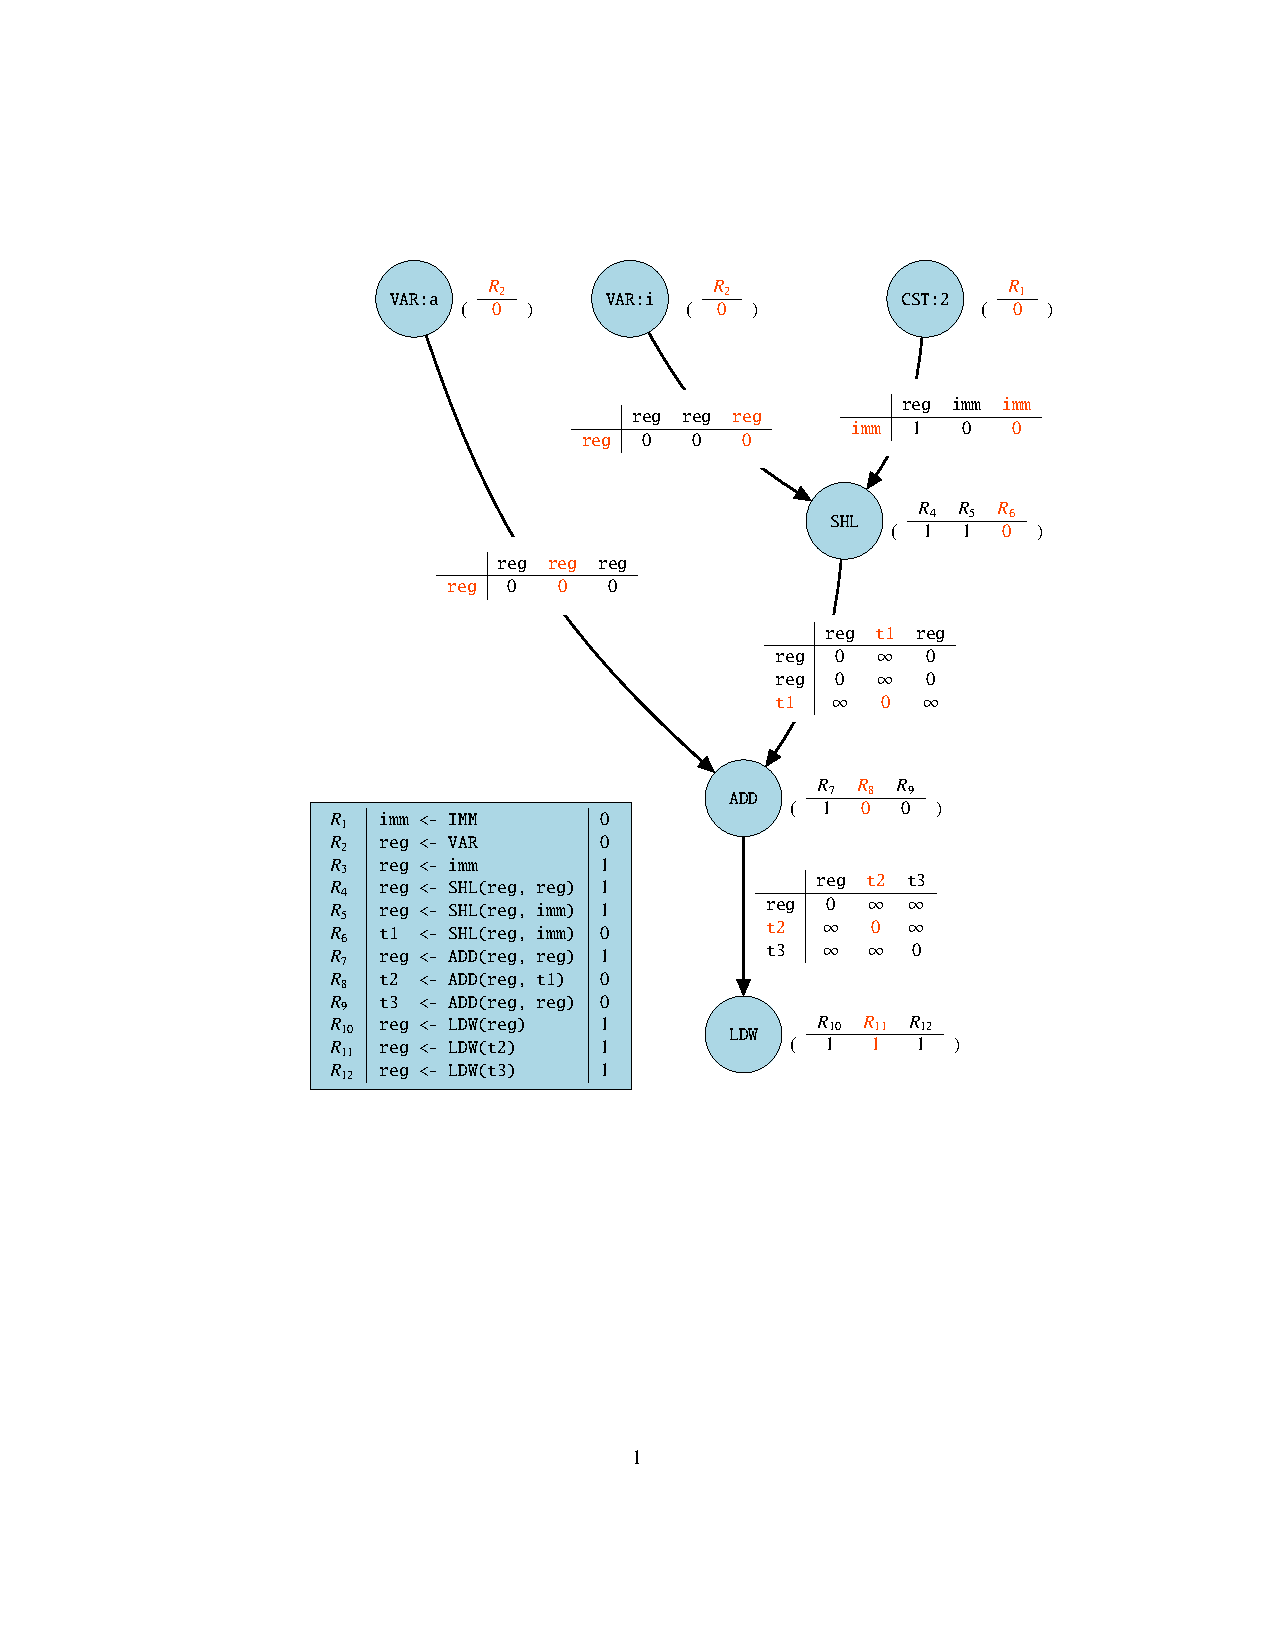
\includegraphics{pgf-fig006}
  \end{center}
  \caption{PBQP instance derived from the example shown in
    Figure~\ref{fig:tpm}. The grammar has been normalized by
    introducing additional nonterminals.}\label{fig:pbpq-example}
\end{figure}

To illustrate this transformation, consider the grammar in
Figure~\ref{fig:pbpq-example}, which is a normalized version of the
tree grammar introduced in Figure~\ref{fig:tpm}. Temporary nonterminal
symbols $\texttt{t1}$, $\texttt{t2}$, and $\texttt{t3}$ are used to
decompose larger tree patterns into simple base rules. Each of these
base rules spans across a single node in the SSA graph.

The instruction selection problem for SSA graphs is modeled in PBQP as
follows. For each node $u$ in the SSA graph, a PBQP variable $x_u$ is
introduced. The domain of variable $x_u$ is determined by the subset
of base rules whose terminal symbol matches the operation of the SSA
node, \eg, there are three rules ($R_4$, $R_5$, $R_6$) that can be
used to cover the shift operation $\texttt{SHL}$ in our example. The
last rule is the result of automatic normalization of a more complex
tree pattern.

The cost vector $\vec{c_u}= w_u \cdot \langle c(R_1), \dots,
c(R_{k_u}) \rangle$ of variable $x_u$ encodes the local costs for a
particular assignment where $c(R_i)$ denotes the associated cost of
base rule $R_i$. Weight $w_u$ is used as a parameter to optimize for
various objectives including speed (e.g. $w_u$ is the expected
execution frequency of the operation at node $u$) and space (e.g. the
$w_u$ is set to one). In our example, both $R_4$ and $R_5$ have
associated costs of one. Rule $R_6$ contributes no local costs as we
account for the full costs of a complex tree pattern at the root
node. All nodes have the same weight of one, thus the cost vector for
the \texttt{SHL} node is $\langle1, 1, 0 \rangle$.

An edge in the SSA graph represents data transfer between the result
of an operation $u$, which is the source of the edge, and the operand
$v$ which is the tail of the edge.  To ensure consistency among base
rules and to account for the costs of chain rules, we impose costs
dependent on the selection of variable $x_u$ and variable $x_v$ in the
form of a cost matrix $\matrixfont C_{uv}$. An element in the matrix
corresponds to the costs of selecting a specific base rule $r_u \in
R_u$ of the result and a specific base rule $r_v \in R_v$ of the
operand node. Assume that $r_u $ is $\texttt{nt} \leftarrow
\textit{op} (\dots)$ and $r_v$ is $\dots \leftarrow \textit{op}
(\alpha, \texttt{nt}', \beta)$ where $\texttt{nt'}$ is the
non-terminal of operand $v$ whose value is obtained from the result of
node $u$. There are three possible cases:
\begin{enumerate}
\item If the nonterminal \texttt{nt} and \texttt{nt}' are identical,
  the corresponding element in matrix $\matrixfont C_{uv}$ is zero,
  since the result of $u$ is compatible with the operand of node $v$.
\item If the nonterminals \texttt{nt} and $\texttt{nt}'$ differ and
  there exists a rule $r: \texttt{nt}' \leftarrow \texttt{nt}$ in the
  transitive closure of all chain-rules, the corresponding element in
  $\matrixfont C_{uv}$ has the costs of the chain rule, \ie $w_v \cdot
  c(r)$.
\item Otherwise, the corresponding element in $\matrixfont C_{uv}$ has
  infinite costs prohibiting the selection of incompatible base rules.
\end{enumerate}

As an example, consider the edge from \texttt{CST:2} to node
\texttt{SHL} in Figure~\ref{fig:pbpq-example}. There is a single base
rule $R_1$ with local costs 0 and result nonterminal \texttt{imm} for
the constant. Base rules $R_4$, $R_5$, and $R_6$ are applicable for
the shift, of which the first one expects nonterminal \texttt{reg} as
its second argument, rules $R_5$ and $R_6$ both expect
\texttt{imm}. Consequently, the corresponding cost matrix accounts for
the costs of converting from \texttt{reg} to \texttt{imm} at index
$(1,1)$ and is zero otherwise.

Highlighted elements in Figure~\ref{fig:pbpq-example} show a
cost-minimal solution of the PBQP with costs one. A solution of the
PBQP directly induces a selection of base and chain rules for the SSA
graph. A traversal over the basic blocks using the SSA graph is
sufficient to execute the associated semantic rules in order to emit
the code.

\section{Extensions and Generalizations}

\subsection{Code Selection for DAG Patterns}
\label{sec:dag_patterns}
% generalization for DAG patterns; motivation; modeling; example
In the previous section we have introduced an approach whose
patterns resemble simple tree fragments, \eg, there is not support for
machine instructions with multiple results. This restricts the
modeling of advanced features commonly found in embedded
architectures and SIMD extensions of nowadays CPUs.

Consider the introductory example shown
in Figure~\ref{fig:ssa_graph}. Most architectures have some form of
auto-increment addressing modes. On such a machine, the load and the
increment of both \texttt{p} and \texttt{q} can be done in a single
instruction benefiting both code size and performance. However,
post-increment loads cannot be modeled using a single tree-shaped
pattern. Instead, it produces multiple results and spans across two
non-adjacent nodes in the SSA graph, with the only restriction that
their arguments have to be the same.

Similar examples can be found in most architectures, \eg, the
\texttt{DIVU} instruction in the Motorola 68K architecture performs
the division and the modulo operation for the same pair of
inputs. Other examples are the \texttt{RMS} (read-modify-store)
instructions on the IA32/AMD64 architecture, autoincrement- and
decrement addressing modes of several embedded systems architectures,
the \texttt{IRC} instruction of the HPPA architecture, or
\texttt{fsincos} instructions of various math libraries. Compiler
writers are forced to pre- or post-process these patterns
heuristically often missing much of the optimization potential
\cite{Ebner08}. These architecture-specific tweaks also complicate
re-targeting, especially in situations where patterns are
automatically derived from generic architecture descriptions.

Supporting these patterns, however, is complicated by dependency
constraints among complex patterns. For any graph cover, the existence
of a topological order is necessary in order to generate correct
code. Cycles would imply that operations are executed on the target
hardware before the values of the operands are available. The partial
order among nodes is defined by the edges in the SSA graph and
eventual memory dependencies.

\begin{figure}
  \begin{center}
    \begin{tabular}{cc}
      \begin{minipage}[c]{4cm}
        \begin{tabbing}
          xx\=xxx\=xxx\=xxx\=\kill
          \texttt{(1) x$_\texttt{1}$:=*p;} \\
          \texttt{(2) *q:=1;} \\
          \texttt{(3) x$_\texttt{2}$:=x$_\texttt{1}$+1;} \\
          \texttt{(4) *p:=x$_\texttt{2}$;}
        \end{tabbing}
      \end{minipage}
      &
      \begin{minipage}[c]{\linewidth-4cm}
        \centering
%         \begin{tikzpicture}
%           \matrix [draw, rounded corners, fill=LightGrey, inner sep=10pt] (m) {
%             \node [fnode, inner sep=0] (st1) {\texttt{ST}};
%             \node [fnode, inner sep=0, below right of=st1, node distance=1.5cm] (inc) {\texttt{INC}};
%             \node [fnode, inner sep=5pt, below left of=inc, node distance=1.5cm] (ld) {\texttt{LD}};
%             \\
%           };

%           \node [fnode, below left of=ld,node distance=2.5cm] (p) {\texttt{VAR:p}} ;
%           \node [fnode, below right of=ld, node distance=2.5cm,xshift=1.5cm] (st2) {\texttt{ST}};
%           \node [fnode, below left of=st2] (q) {\texttt{VAR:q}};
%           \node [fnode, below right of=st2] (1) {\texttt{1}};

%           \path (m.north west) node [anchor=south west] {RMS Pattern};
%           \path [arrow,->] (ld) -- (inc);
%           \path [arrow,->] (inc) -- (st1);
%           \path [arrow,->] (1) -- (st2);
%           \path [arrow,->] (q) -- (st2);
%           \path [arrow,->] (p) -- (ld);
%           \path [arrow,->] (p) edge [bend left=20] (st1);

%           \node [below right of=ld,node distance=1.5cm] (c1) {};
%           \node [left of=st2,node distance=1cm,yshift=0.5cm] (c2) {};
%           \path [arrow,dashed,->] (ld) .. controls (c1.center) and
%           (c2.center) .. node [fill=white] {\texttt{WAR}}  (st2);

%           \node [above  of=st2,node distance=2cm,xshift=10pt] (c1) {};
%           \node [right of=st1,node distance=3.5cm] (c2) {};
%           \path [arrow,dashed,->] (st2) .. controls (c1.center) and
%           (c2.center) .. node [fill=white] {\texttt{WAW}}  (st1);
%         \end{tikzpicture}
        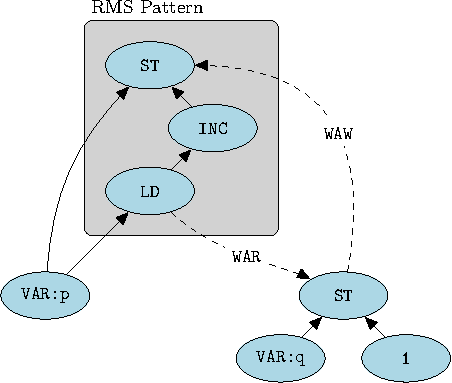
\includegraphics{pgf-fig007}
      \end{minipage}
      \\
      \\
      (a) Input Block &  (b) SSA Graph \\
    \end{tabular}
  \end{center}
  \caption{Potential memory dependencies for a tree-shaped
    read-modify-store (RMS) pattern.}\label{fig:rms}
\end{figure}

In principle, such issues can even arise for tree-shaped patterns. An
example is given in Figure~\ref{fig:rms}, which shows a typical
read-modify-store (RMS) pattern (``\texttt{add~r/m32,~imm32}'') for
the IA32/AMD64 architecture. A corresponding production rule might be
formulated as
\begin{alltt}
  stmt <- ST(\textit{x}:reg, ADD(LD(\textit{x}), imm)).
\end{alltt}
If we have to assume that \texttt{p} and \texttt{q} might address the
same memory location, we have to account for the antidependency among
statements \texttt{(1)} and \texttt{(2)} and the output dependency
among statements \texttt{(2)} and \texttt{(4)}; depicted in
Figure~\ref{fig:rms}\emph{(b)\/} by dotted lines. There is obviously
no topological order among the highlighted part forming the RMS
pattern and the store corresponding to instruction~\texttt{(2)}. Thus,
we cannot apply the pattern without introducing cyclic dependencies.

\begin{figure}[t]
  \centering
%   \begin{tikzpicture}

%     \node [anchor=south west] at (-5cm, 1cm) (listing) {
%       \begin{minipage}[]{7cm}
%         \begin{tabbing}
%           xx\=xxx\=xxx\=xxx\=\kill
%           \texttt{*p:=r+1;} \\
%           \texttt{*q:=p+1;} \\
%           \texttt{*r:=q+1;} \\
%         \end{tabbing}
%       \end{minipage}
%     };

%     \tikzstyle{mstyle}= [matrix,draw, fill=LightGrey, rounded
%     corners,column sep=10pt,row sep=10pt,inner sep=8pt];
%     \node[regular polygon, regular polygon sides=3, minimum size=4.5cm] (frame) {};

%     \path (frame.corner 2) node [mstyle] (m1) {
%       \node [fnode, inner sep=0] (st1) {\texttt{ST}}; \\
%       \node [fnode, inner sep=0] (inc1) {\texttt{INC}}; \\
%     };

%     \path (frame.corner 3) node [mstyle] (m2) {
%       \node [fnode, inner sep=0] (inc2) {\texttt{INC}}; \\
%       \node [fnode, inner sep=0] (st2) {\texttt{ST}}; \\
%     };

%     \path (frame.corner 1) node [mstyle, yshift=-0.8cm] (m3) {
%       \node [fnode, inner sep=0] (inc3) {\texttt{INC}}; &
%       \node [fnode, inner sep=0] (st3) {\texttt{ST}}; \\
%     };

%     \node [fnode, left of=m1,node distance=2.5cm] (q) {\texttt{VAR:q}};
%     \node [fnode, right of=m2,node distance=2.5cm] (r) {\texttt{VAR:r}};
%     \node [fnode, above of= m3,node distance=1.5cm] (p) {\texttt{VAR:p}};

%     \path [arrow,->] (inc1) -- (st2);
%     \path [arrow,->] (inc2) edge[bend right=15pt] (st3);
%     \path [arrow,->] (inc3) edge[bend right=15pt] (st1);

%     \path [arrow,->] (q) edge[bend right=5pt] (inc1);
%     \path [arrow,->] (q) edge[bend left=5pt] (st1);
%     \path [arrow,->] (r) edge[bend left=5pt] (st2);
%     \path [arrow,->] (r) edge[bend right=5pt] (inc2);
%     \path [arrow,->] (p) edge[bend right=5pt] (inc3);
%     \path [arrow,->] (p) edge[bend left=5pt] (st3);

%   \end{tikzpicture}
    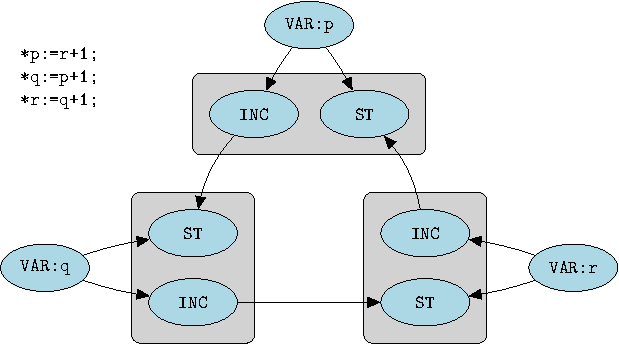
\includegraphics{pgf-fig008}
  \caption{DAG patterns may introduce cyclic data dependencies.}\label{fig:topology}
\end{figure}

However, for tree-shaped patterns, we can always perform a
\emph{local} check that determines if a particular pattern is or is
not applicable. For DAG patterns, this is not necessarily the
case. Again, an example is given in Figure~\ref{fig:topology}.  The
code fragment contains three feasible examples of a post-increment
store pattern. Assuming that we know that $p$, $q$, and $r$ point to
mutually distinct memory locations, there are no further dependencies
apart from the edges shown in the SSA graph.  However, the situation
is now different.  The example gives rise to a topological order as
long as we do not select \emph{all} three instances of the
post-increment store pattern concurrently. Thus, the existence of a
topological order is now a global property, which has to be considered
in the modeling of the problem.

\begin{algorithm}
\caption{Generalized PBQP instruction selection}
\label{alg:pbqpisel}
\begin{algorithmic}[1]
  \STATE identify instances of complex patterns within basic blocks
  \STATE transform the problem to an instance of PBQP
  \STATE obtain a solution for the PBQP instance using a generic
  solver
  \FORALL{basic blocks $b$}
    \STATE compute a topological order for the subgraph
    induced by basic block $b$
    \STATE apply the semantic rules associated with the chosen
    productions in the order computed in step \texttt{(5)}.
  \ENDFOR
\end{algorithmic}
\end{algorithm}

A proper generalization of the PBQP based instruction selection
\cite{Ebner08} is outlined in Algorithm~\ref{alg:pbqpisel}. Only steps
\texttt{(1)}, \texttt{(2)}, and \texttt{(5)} differ from the approach
discussed so far. First, we identify concrete tuples of nodes in the
SSA graph that can be used to form complex patterns. Next, we
transform the problem to an instance of PBQP that is processed using a
generic solver library. The problem formulation ensures the existence
of a topological order among the chosen productions and allows for a
straight-forward back-transformation that maps a solution vector of
PBQP to a complete graph cover. The partial order among the particular
nodes is defined by the edges in the SSA graph and additional data
dependencies among load and store instructions.  We can thus use a
reversed post-order traversal to apply the semantic actions associated
with the chosen productions in a proper order on the subgraphs induced
by individual basic blocks.

\subsubsection{Modeling.}
As for tree patterns, DAG patterns are decomposed into simple base
rules for the purpose of modeling, \eg, the postincrement store
pattern
\begin{alltt}
  P1: tmt <- ST(\textit{x}:reg, reg), reg <- INC(\textit{x}) : 3
\end{alltt}
is decomposed into the individual pattern fragments
\begin{alltt}
  P1.1: stmt <- ST(reg, reg)
  P1.2: reg  <- INC(reg)
\end{alltt}
The matcher explicitly enumerates \emph{instances\/} of complex
patterns in step \texttt{(1)} of Algorithm~\ref{alg:pbqpisel}, \ie,
concrete tuples of nodes that match the terminal symbols specified in
a particular production. In the example shown in
Figure~\ref{fig:topology}, there are three instances of the
postincrement store pattern. Dependencies among these instances
(denoted in the following by $\prec$) arise from real dependencies
among individual nodes (edges in the SSA graph) and eventual memory
dependencies as outlined in Figure~\ref{fig:rms}.

For instances of DAG patterns, additional decision variables are
required that encode if the particular pattern is to be
selected. Thus, we have two sets of decision variables
$X=X_1~\dotcup~X_2$ for regular SSA nodes and instances of complex
patterns respectively.

The domain for variables in $X_1$ is defined by the set of applicable
base rules arising from two different sources:
\begin{enumerate}
\item Simple productions consisting of a single base rule; these are
  handled just like before for tree grammars.
\item Base rules arising from the decomposition of DAG patterns. All
  identical base rules obtained from the decomposition of complex
  productions contribute only to a single element in the decision
  vector.
\end{enumerate}
While the former group represents the set of simple patterns that can
be used to obtain a cover for a particular node, the second class of
base rules can be seen as a proxy for the whole set of instances of
(possibly different) complex productions including the node. The
costs for these proxy states are $0$, otherwise they reflect the
real costs of the corresponding tree rule.

Variables in set $X_2$ are created for each enumerated instance of a
complex production. They encode whether a particular instance is
chosen or not, \ie, the domain basically consists of the elements
\textit{on} and \textit{off}. The local costs reflect the costs for
the particular pattern except for the \textit{off} state, which is set
to $0$.

\begin{figure}
  \centering
%   \begin{tikzpicture}[]

%     \tikzstyle{mstyle}= [matrix,draw, fill=LightGrey, rounded corners,
%     column sep=10pt,row sep=10pt,inner sep=8pt];
%     \tikzstyle{nstyle}= [draw,fill=LightBlue,shape=rectangle,rounded corners,inner sep=2pt];

%     \node[regular polygon, regular polygon sides=3, minimum size=3.3cm] (frame) {};

%     \path (frame.corner 1) +(0,0) node  (ci1) [nstyle, yshift=0.6cm]
%     {
%       \begin{tabular}{@{}c@{}}
%         7: instance $\langle 2,1 \rangle$ \\
%         \hline
%         $\begin{array}{cccccc}
%           & \texttt{off} & \texttt{on}_1 & \texttt{on}_2 & \texttt{on}_3 & \\
%           ( & 0 & k & k & k & )
%         \end{array}$
%       \end{tabular}
%     };

%     \path (frame.corner 2) +(-1.5,0) node  (ci2) [nstyle]
%     {
%       \begin{tabular}{@{}c@{}}
%         8: instance $\langle 3,4 \rangle$ \\
%         \hline
%         $\begin{array}{cccccc}
%           & \texttt{off} & \texttt{on}_1 & \texttt{on}_2 & \texttt{on}_3 & \\
%           ( & 0 & k & k & k & )
%         \end{array}$
%       \end{tabular}
%     };

%     \path (frame.corner 3) +(1.5,0) node  (ci3) [nstyle]
%     {
%       \begin{tabular}{@{}c@{}}
%         9: instance $\langle 5,6 \rangle$ \\
%         \hline
%         $\begin{array}{cccccc}
%           & \texttt{off} & \texttt{on}_1 & \texttt{on}_2 & \texttt{on}_3 & \\
%           ( & 0 & k & k & k & )
%         \end{array}$
%       \end{tabular}
%     };

%     \path (frame.corner 2) +(-1,-4.5) node [mstyle] (m1)
%     {
%       \node  (st1) [nstyle]
%       {
%         \begin{tabular}{@{}c@{}}
%           3: \texttt{ST} \\
%           \hline
%           $(\, \texttt{P2} \quad \texttt{P1.1}\, )$\\
%           $(\, 2 \quad \texttt{M} \,)$ \\
%         \end{tabular}
%       };
%       &

%       \node  (inc1) [nstyle]
%       {
%         \begin{tabular}{@{}c@{}}
%           4: \texttt{INC} \\
%           \hline
%           $(\, \texttt{P3} \quad \texttt{P1.2}\, )$\\
%           $(\, 2 \quad \texttt{M} \,)$ \\
%         \end{tabular}
%       };

%       \\
%     };

%     \path (frame.corner 3) +(1,-4.5) node [mstyle] (m2)
%     {
%       \node  (st2) [nstyle]
%       {
%         \begin{tabular}{@{}c@{}}
%           5: \texttt{ST} \\
%           \hline
%           $(\, \texttt{P2} \quad \texttt{P1.1}\, )$\\
%           $(\, 2 \quad \texttt{M} \,)$ \\
%         \end{tabular}
%       };
%       &

%       \node  (inc2) [nstyle]
%       {
%         \begin{tabular}{@{}c@{}}
%           6: \texttt{INC} \\
%           \hline
%           $(\, \texttt{P3} \quad \texttt{P1.2}\, )$\\
%           $(\, 2 \quad \texttt{M} \,)$ \\
%         \end{tabular}
%       }; \\
%     };

%     \path (frame.corner 1) +(0,4.5) node [mstyle] (m3)
%     {
%       \node  (inc3) [nstyle]
%       {
%         \begin{tabular}{@{}c@{}}
%           1: \texttt{INC} \\
%           \hline
%           $(\, \texttt{P3} \quad \texttt{P1.2}\, )$\\
%           $(\, 2 \quad \texttt{M} \,)$ \\
%         \end{tabular}
%       };
%       &
%       \node  (st3) [nstyle]
%       {
%         \begin{tabular}{@{}c@{}}
%           2: \texttt{ST} \\
%           \hline
%           $(\, \texttt{P2} \quad \texttt{P1.1}\, )$\\
%           $(\, 2 \quad \texttt{M} \,)$ \\
%         \end{tabular}
%       };
%       \\
%     };

%     \node [fnode, below of=m1,node distance=1.8cm] (q) {\texttt{VAR:q}};
%     \node [fnode, below of=m2,node distance=1.8cm] (r) {\texttt{VAR:r}};
%     \node [fnode, above of=m3,node distance=1.8cm] (p) {\texttt{VAR:p}};

%     \path [arrow,->] (q) -- (inc1);
%     \path [arrow,->] (q) -- (st1);
%     \path [arrow,->] (r) -- (st2);
%     \path [arrow,->] (r) -- (inc2);
%     \path [arrow,->] (p) -- (inc3);
%     \path [arrow,->] (p) -- (st3);

%     \path[arrow,->] (inc1) edge[bend right=60pt] node[yshift=-0.6cm] {$\left( { \begin{array}{cc}
%             0 & 0 \\
%             0 & 0 \\
%           \end{array}} \right)$} (st2);

%     \path [arrow,->] (inc2.east) .. controls
%     ($(inc2)+(3.2cm,2cm)$) and ($(st3)+(4cm,-2cm)$) ..
%     node[fill=white,near end] {$\left( { \begin{array}{cc}
%             0 & 0 \\
%             0 & 0 \\
%           \end{array}} \right)$} (st3.east);

%     \path [arrow,->] (inc3.west) .. controls ($(inc3)+(-4cm,-2cm)$) and
%     ($(st1)+(-3.2cm,2cm)$) ..
%     node[fill=white,near start] {$\left( { \begin{array}{cc}
%             0 & 0 \\
%             0 & 0 \\
%           \end{array}} \right)$} (st1.west);

%     \path[arrow,->] (ci2) edge[bend right=10] node[fill=white] {$\left( { \begin{array}{cccc}
%             0 & 0 & 0 & 0 \\
%             0 & \infty & 0 & 0 \\
%             0 & \infty & \infty & 0 \\
%             0 & \infty & \infty & \infty \\
%           \end{array}} \right)$} (ci3);

%     \path[arrow,->] (ci3) edge[bend right=60] node[fill=white] {$\left( { \begin{array}{cccc}
%             0 & 0 & 0 & 0 \\
%             0 & \infty & 0 & 0 \\
%             0 & \infty & \infty & 0 \\
%             0 & \infty & \infty & \infty \\
%           \end{array}} \right)$} (ci1.east);

%     \path[arrow,<-] (ci2) edge[bend left=60] node[fill=white] {$\left( { \begin{array}{cccc}
%             0 & 0 & 0 & 0 \\
%             0 & \infty & 0 & 0 \\
%             0 & \infty & \infty & 0 \\
%             0 & \infty & \infty & \infty \\
%           \end{array}} \right)$} (ci1.west);

%     \path[arrow,->] (inc3) edge[bend right=30] node[fill=white] {$\left( { \begin{array}{cccc}
%             0 & \infty & \infty & \infty \\
%             0 & 0 & 0 & 0 \\
%           \end{array}} \right)$} (ci1);


%     \path[arrow,->] (st3) edge[bend left=30] node[fill=white] {$\left( { \begin{array}{cccc}
%             0 & \infty & \infty & \infty \\
%             0 & 0 & 0 & 0 \\
%           \end{array}} \right)$} (ci1);


%     \path[arrow,->] (inc1) edge[bend right=30] node[fill=white] {$\left( { \begin{array}{cccc}
%             0 & \infty & \infty & \infty \\
%             0 & 0 & 0 & 0 \\
%           \end{array}} \right)$} (ci2);


%     \path[arrow,->] (st1) edge[bend left=30] node[fill=white] {$\left( { \begin{array}{cccc}
%             0 & \infty & \infty & \infty \\
%             0 & 0 & 0 & 0 \\
%           \end{array}} \right)$} (ci2);

%     \path[arrow,->] (inc2) edge[bend right=30] node[fill=white] {$\left( { \begin{array}{cccc}
%             0 & \infty & \infty & \infty \\
%             0 & 0 & 0 & 0 \\
%           \end{array}} \right)$} (ci3);


%     \path[arrow,->] (st2) edge[bend left=30] node[fill=white] {$\left( { \begin{array}{cccc}
%             0 & \infty & \infty & \infty \\
%             0 & 0 & 0 & 0 \\
%           \end{array}} \right)$} (ci3);


%   \end{tikzpicture}
    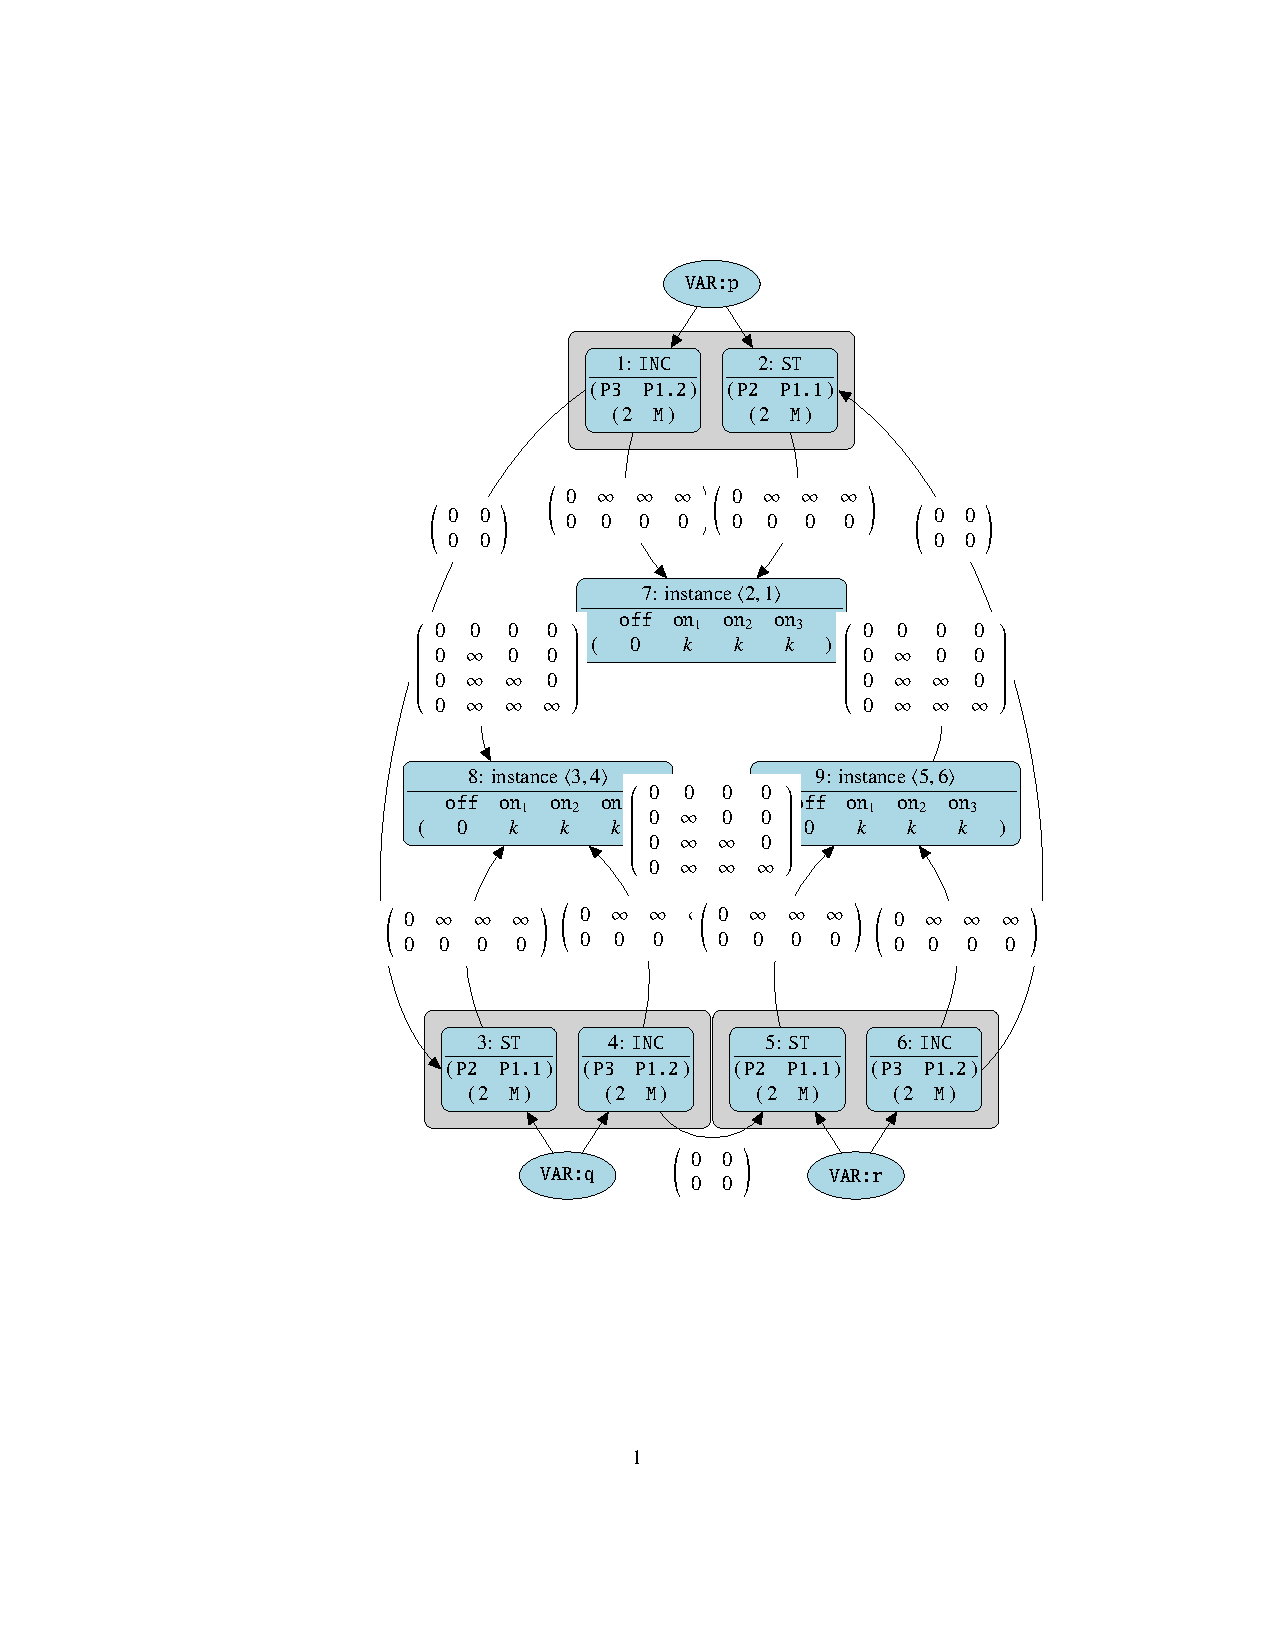
\includegraphics{pgf-fig009}
  \caption{PBQP Graph for the Example shown in
    Figure~\ref{fig:topology}. We use $k$ as a shorthand for the term
    $3-2M$.}\label{fig:pbqpinst}
\end{figure}

The PBQP for the SSA graph introduced in Figure~\ref{fig:topology} is
shown in Figure~\ref{fig:pbqpinst}. In addition to the postincrement
store pattern with costs 3, we assume regular tree patterns for the
store and the increment nodes with costs two denoted by \texttt{P2}
and \texttt{P3} respectively. Rules for the \texttt{VAR} nodes are
omitted for simplicity.

Nodes one to six correspond to the nodes in the SSA graph. Their
domain is defined by the simple base rule with costs two and the proxy
state obtained from the decomposition of the postincrement store
pattern. Nodes 7, 8, and 9 correspond to the three instances
identified for the postincrement store pattern. As noted before, we
have to to guarantee the existence of a topological order among the
chosen nodes.  One approach is to exploit the property that every
acyclic directed subgraph gives rise to a not necessarily unique
topological order.  We can refine the state \textit{on} such that it
reflects a particular index in a concrete topological order. Matrices
among these nodes account for data dependencies, \eg, consider the
matrix established among nodes 7 and 8. Assuming instance 7 is
\textit{on} at index 2, The only remaining choices for instance 8 are
not to use the pattern or to enable it at index three, as node 7 has
to precede node 8.

A different class of constraint matrices is required to ensure that
the corresponding proxy state is selected on all the variables forming
a particular pattern instance. Therefore, we create matrix costs
$C^{X_1 \rightarrow X_2}_{ul}$ such that the costs are zero if $x_l$
is set to \textit{off\/} or $x_u$ is set to a base rule that is not
associated to the instance. Otherwise, costs are set to $\infty$.
Thus, when one of the instances correlated to a particular node $u$ in
the SSA graph is selected, the only remaining element in the domain of
$u$ with costs less than $\infty$ is the associated proxy state
corresponding to the particular base rule fragment.

So far, the formulation allows the trivial solution where all of the
related variables encoding the selection of a complex pattern are set
to \textit{off} (accounting for 0 costs) even though the artificial
proxy state has been selected. We can overcome this problem by adding
a large integer value $M$ to the costs for all proxy states. In
exchange, we subtract these costs from the cost vector of
instances. Thus, the penalties for the proxy states are effectively
eliminated unless an invalid solution is selected.

Cost matrices among nodes one to six do not differ from the basic
approach discussed before and reflect the costs of converting the
nonterminal symbols involved.

It should be noted that for general grammars and irreducible graphs,
the heuristic algorithm proposed in Section~\ref{sec:pbqp:heuristic}
cannot be guaranteed to deliver a solution that satisfies all
constraints modeled in terms of $\infty$ costs. This would be a
NP-complete problem. One way to work around this limitation is to
include a small set of rules that cover each node individually and
that can be used as a fallback rule in situations where no feasible
solution has been obtained. This corresponds to macro substitution
techniques and ensures a correct but possibly suboptimal matching. In
practice, this is no severe limitation as grammars are usually written
by defining a simple but complete set of rules covering each node
individually and adding more complex rules later on. These limitations
do not apply to exact techniques such as the branch-\&-bound algorithm
introduced in Section~\ref{sec:pbqp:bab}. It is also straight-forward
to extend the heuristic algorithm with a backtracking scheme on RN
reductions, which would clearly also be exponential in the worst case.

\subsection{Chain Rule Placement}
\label{sec:chain_rule_placement}
% \emph{1 page}; optimal chain rule placement
Chain rules can either be emitted at the basic block corresponding to
the source node or right before each use, \ie, at the destination
node. In~\cite{1269857}, a more sophisticated technique is introduced
that allows a more efficient placement of chain rules across basic
block boundaries. This technique is orthogonal to the generalization
to complex patterns. An optimal placement is computed by the
construction of a min-cut problem for the given control flow graph. A
solution for this problem can be found in polynomial time. There is a
trade-off among performance and code size that is captured accurately
in the proposed network flow model.

Consider the example in Figure~\ref{fig:crp-example}(a) which shows a
fraction of the control flow graph. The nodes of the graph represent
basic blocks in the control flow graph and edges represent flow of
control between basic blocks. Execution frequencies are given for each
basic block which are obtained by profiling. Assume that the example
is in pruned SSA form, and in node $d$ is a definition of the form
\texttt{x$_0$ = ...} and in node $u$ is a use of the definition
\texttt{...x$_0$...}. For a given graph grammar, let's assume we need
to place a chain rule that has to be executed at least once on all
paths from $d$ to $u$. To find a cost optimal placement, we reduce the
problem to an $s-t$ min cut as shown in the
Figure~\ref{fig:crp-example}(b). Each node $v$ in the control flow
graph corresponds to two vertices $v_e$ and $v_x$ in the network of
the $s-t$ min cut. An edge between $v_e$ and $v_x$ represents the cost
of placing the chain rule in node $v$.  For each edge $(v,w)$ in the
control flow graph, there exists an edge $(v_x,w_e)$ in the network
that has infinite cost weights. Nodes $s$ and $t$ have connections to
the definition node $d_e$ and the use node $u_x$ respectively. A cut
of such a network can only consists of edges $(v_e,v_x)$ because all
other edges have infinite costs. All cut edges represent nodes where
we can place chain rules rules optimally and ensure that on all paths
from $d$ to $u$ the chain rule is executed. An $s-t$ min cut of the
newly constructed network, gives us an optimal placement of chain
rules. For the example the optimal cut is node $b$ since $(b_e,b_x)$
separates node $s$ from node $t$ in the network with only a single
cost unit.


\begin{figure}
\begin{center}
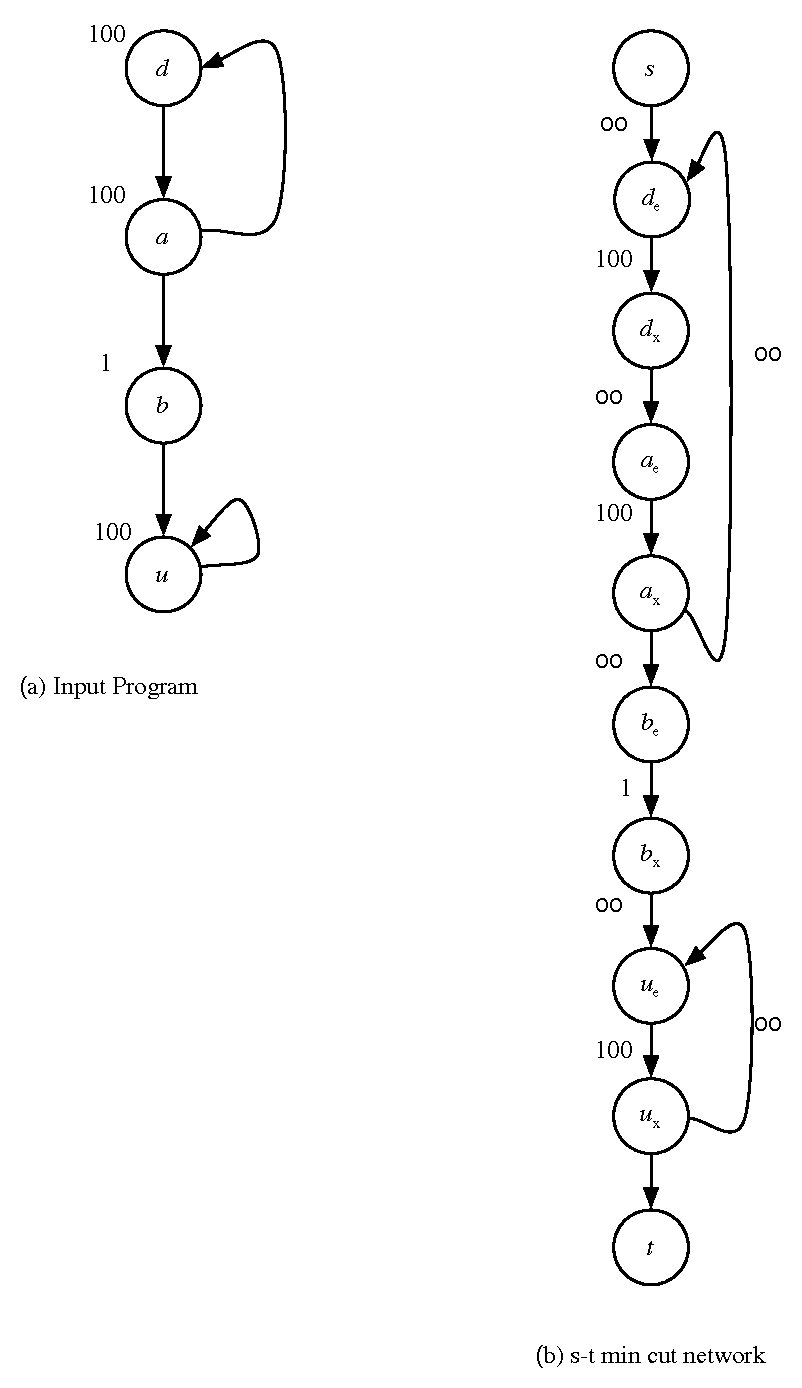
\includegraphics[width=0.5\textwidth]{Example.pdf}
\end{center}
\caption{Example for Chain Rule Placement}\label{fig:crp-example}
\end{figure}

%%% Local Variables:
%%% mode: latex
%%% TeX-master: "chapter"
%%% End:
